\chapter{Results}

This chapter presents the findings of the experiments conducted in this master's thesis. The chapter is divided into two sections.
The first section presents the results of \methodOne{1}, and the second section presents the results of \methodTwo{2}, where both methods will be evaluated in the context of both Gaussian VAEs and VQ-VAEs. In the final section, I will present the cross-validation results of both methods.

\section{Results of \methodOne{1}}

In this section, I will present the results of \methodOne{1} on both Gaussian VAEs and VQ-VAEs.

\subsection{Results on Gaussian VAEs}

The experiments showed similar results for both exact sampling and uniform sampling. The results showed that \methodOne{1} can be used not only to obtain a conditioned decoder but also to improve the quality of non-conditioned decoder reconstruction when compared to non-conditioned Gaussian VAEs. However, KL divergence loss of the latent space increased when \methodOne{1} was applied. This can be explained by the fact that there is a trade-off between the quality of the reconstruction and the KL divergence of the latent space. An example of this can be seen in figure \ref{fig:results_method1_gaussian_vae}. 

The reconstruction loss of the conditioned decoder was improved when compared to the non-conditioned decoder \ref{fig:res_val}.

To validate and verify that the results are not influenced due to the architecture of the neural network, I applied a range of loss-balancing techniques such as coefficient balancing and the SoftAdapt algorithm. After applying these techniques it could still be observed that the quality of the reconstruction was improved at the expense of a slightly higher KL divergence loss of the latent space. When comparing the results of the Exact Same Sampling and Uniform Sampling it showed little difference to each other.

When trying to use deeper neural networks on the Gaussian VAEs, I observed that the posterior collapse was more likely to happen, which is a common problem in Gaussian VAEs~\cite{wang2023posterior}.
% Think about Coefficients the number of pixels to be sampled. How it changes the results.

\begin{figure}[H]
    \centering
    \centering
\scriptsize
\begin{tabular}{||c|c|c|c||}
\hline
 Method & Parameters & Reconstruction loss & KL loss \\
\hline
\textit{Baseline} & - & 0.0042 +- 1.2e-03 & 0.0018 +- 6.3e-04 \\
\hline
Multi Decoder & Exact sampling & 0.0036 +- 8.3e-04  $\downarrow$ & 0.0027 +- 8.7e-04  $\uparrow$ \\
\hline
Multi Decoder & Exact sampling, SoftAdapt & 0.0034 +- 1.9e-04  $\downarrow$ & 0.0029 +- 2.8e-03  $\uparrow$ \\
\hline
Multi Decoder & Uniform sampling & 0.0035 +- 6.5e-04  $\downarrow$ & 0.0026 +- 1.7e-03  $\uparrow$ \\
\hline
Multi Decoder & Uniform sampling, SoftAdapt & 0.0034 +- 7.3e-03  $\downarrow$ & 0.0029 +- 2.0e-02  $\uparrow$ \\
\hline
\end{tabular}

    \caption[Trained neural network with \methodOne{1} applied to a Gaussian VAE.]
    { 
        Trained neural network with \methodOne{1} with Exact Same Sampling applied to a Gaussian VAE on CelebA dataset and latent space 16. 
        On the left side as input is the original image, on the right side there are two outputs of the decoders. 
        The image from the conditioned decoder is reconstructed with higher quality compared to the non-conditioned decoder because the conditioned decoder $Decoder_2$ uses conditioning information $m$ to improve the quality of the reconstruction.
    }
    \label{fig:res_val}
\end{figure}


\begin{figure}[H]
    \centering
    \scalebox{0.48}{%% Creator: Matplotlib, PGF backend
%%
%% To include the figure in your LaTeX document, write
%%   \input{<filename>.pgf}
%%
%% Make sure the required packages are loaded in your preamble
%%   \usepackage{pgf}
%%
%% Also ensure that all the required font packages are loaded; for instance,
%% the lmodern package is sometimes necessary when using math font.
%%   \usepackage{lmodern}
%%
%% Figures using additional raster images can only be included by \input if
%% they are in the same directory as the main LaTeX file. For loading figures
%% from other directories you can use the `import` package
%%   \usepackage{import}
%%
%% and then include the figures with
%%   \import{<path to file>}{<filename>.pgf}
%%
%% Matplotlib used the following preamble
%%   
%%   \usepackage{fontspec}
%%   \setmainfont{DejaVuSerif.ttf}[Path=\detokenize{/home/edvardsz/miniconda3/envs/pytorch-latest/lib/python3.10/site-packages/matplotlib/mpl-data/fonts/ttf/}]
%%   \setsansfont{DejaVuSans.ttf}[Path=\detokenize{/home/edvardsz/miniconda3/envs/pytorch-latest/lib/python3.10/site-packages/matplotlib/mpl-data/fonts/ttf/}]
%%   \setmonofont{DejaVuSansMono.ttf}[Path=\detokenize{/home/edvardsz/miniconda3/envs/pytorch-latest/lib/python3.10/site-packages/matplotlib/mpl-data/fonts/ttf/}]
%%   \makeatletter\@ifpackageloaded{underscore}{}{\usepackage[strings]{underscore}}\makeatother
%%
\begingroup%
\makeatletter%
\begin{pgfpicture}%
\pgfpathrectangle{\pgfpointorigin}{\pgfqpoint{6.400000in}{4.800000in}}%
\pgfusepath{use as bounding box, clip}%
\begin{pgfscope}%
\pgfsetbuttcap%
\pgfsetmiterjoin%
\definecolor{currentfill}{rgb}{1.000000,1.000000,1.000000}%
\pgfsetfillcolor{currentfill}%
\pgfsetlinewidth{0.000000pt}%
\definecolor{currentstroke}{rgb}{1.000000,1.000000,1.000000}%
\pgfsetstrokecolor{currentstroke}%
\pgfsetdash{}{0pt}%
\pgfpathmoveto{\pgfqpoint{0.000000in}{0.000000in}}%
\pgfpathlineto{\pgfqpoint{6.400000in}{0.000000in}}%
\pgfpathlineto{\pgfqpoint{6.400000in}{4.800000in}}%
\pgfpathlineto{\pgfqpoint{0.000000in}{4.800000in}}%
\pgfpathlineto{\pgfqpoint{0.000000in}{0.000000in}}%
\pgfpathclose%
\pgfusepath{fill}%
\end{pgfscope}%
\begin{pgfscope}%
\pgfsetbuttcap%
\pgfsetmiterjoin%
\definecolor{currentfill}{rgb}{1.000000,1.000000,1.000000}%
\pgfsetfillcolor{currentfill}%
\pgfsetlinewidth{0.000000pt}%
\definecolor{currentstroke}{rgb}{0.000000,0.000000,0.000000}%
\pgfsetstrokecolor{currentstroke}%
\pgfsetstrokeopacity{0.000000}%
\pgfsetdash{}{0pt}%
\pgfpathmoveto{\pgfqpoint{0.800000in}{0.528000in}}%
\pgfpathlineto{\pgfqpoint{5.760000in}{0.528000in}}%
\pgfpathlineto{\pgfqpoint{5.760000in}{4.224000in}}%
\pgfpathlineto{\pgfqpoint{0.800000in}{4.224000in}}%
\pgfpathlineto{\pgfqpoint{0.800000in}{0.528000in}}%
\pgfpathclose%
\pgfusepath{fill}%
\end{pgfscope}%
\begin{pgfscope}%
\pgfpathrectangle{\pgfqpoint{0.800000in}{0.528000in}}{\pgfqpoint{4.960000in}{3.696000in}}%
\pgfusepath{clip}%
\pgfsetbuttcap%
\pgfsetroundjoin%
\definecolor{currentfill}{rgb}{0.121569,0.466667,0.705882}%
\pgfsetfillcolor{currentfill}%
\pgfsetfillopacity{0.200000}%
\pgfsetlinewidth{0.000000pt}%
\definecolor{currentstroke}{rgb}{0.000000,0.000000,0.000000}%
\pgfsetstrokecolor{currentstroke}%
\pgfsetdash{}{0pt}%
\pgfpathmoveto{\pgfqpoint{1.025455in}{3.929189in}}%
\pgfpathlineto{\pgfqpoint{1.025455in}{3.537991in}}%
\pgfpathlineto{\pgfqpoint{1.071001in}{3.122283in}}%
\pgfpathlineto{\pgfqpoint{1.116547in}{2.832449in}}%
\pgfpathlineto{\pgfqpoint{1.162094in}{2.903462in}}%
\pgfpathlineto{\pgfqpoint{1.207640in}{2.687249in}}%
\pgfpathlineto{\pgfqpoint{1.253186in}{2.916588in}}%
\pgfpathlineto{\pgfqpoint{1.298733in}{3.033231in}}%
\pgfpathlineto{\pgfqpoint{1.344279in}{3.015861in}}%
\pgfpathlineto{\pgfqpoint{1.389826in}{2.836476in}}%
\pgfpathlineto{\pgfqpoint{1.435372in}{3.085044in}}%
\pgfpathlineto{\pgfqpoint{1.480918in}{2.915581in}}%
\pgfpathlineto{\pgfqpoint{1.526465in}{3.127264in}}%
\pgfpathlineto{\pgfqpoint{1.572011in}{3.169460in}}%
\pgfpathlineto{\pgfqpoint{1.617557in}{3.207472in}}%
\pgfpathlineto{\pgfqpoint{1.663104in}{3.187534in}}%
\pgfpathlineto{\pgfqpoint{1.708650in}{3.240190in}}%
\pgfpathlineto{\pgfqpoint{1.754197in}{3.134822in}}%
\pgfpathlineto{\pgfqpoint{1.799743in}{3.259595in}}%
\pgfpathlineto{\pgfqpoint{1.845289in}{3.194550in}}%
\pgfpathlineto{\pgfqpoint{1.890836in}{3.211237in}}%
\pgfpathlineto{\pgfqpoint{1.936382in}{3.121448in}}%
\pgfpathlineto{\pgfqpoint{1.981928in}{3.302009in}}%
\pgfpathlineto{\pgfqpoint{2.027475in}{3.157058in}}%
\pgfpathlineto{\pgfqpoint{2.073021in}{3.193563in}}%
\pgfpathlineto{\pgfqpoint{2.118567in}{3.204020in}}%
\pgfpathlineto{\pgfqpoint{2.164114in}{3.235871in}}%
\pgfpathlineto{\pgfqpoint{2.209660in}{3.219401in}}%
\pgfpathlineto{\pgfqpoint{2.255207in}{3.155879in}}%
\pgfpathlineto{\pgfqpoint{2.300753in}{3.140057in}}%
\pgfpathlineto{\pgfqpoint{2.346299in}{3.276677in}}%
\pgfpathlineto{\pgfqpoint{2.391846in}{3.248486in}}%
\pgfpathlineto{\pgfqpoint{2.437392in}{3.232774in}}%
\pgfpathlineto{\pgfqpoint{2.482938in}{3.120404in}}%
\pgfpathlineto{\pgfqpoint{2.528485in}{3.108912in}}%
\pgfpathlineto{\pgfqpoint{2.574031in}{3.259645in}}%
\pgfpathlineto{\pgfqpoint{2.619578in}{3.191275in}}%
\pgfpathlineto{\pgfqpoint{2.665124in}{3.147473in}}%
\pgfpathlineto{\pgfqpoint{2.710670in}{3.066586in}}%
\pgfpathlineto{\pgfqpoint{2.756217in}{3.010422in}}%
\pgfpathlineto{\pgfqpoint{2.801763in}{3.149030in}}%
\pgfpathlineto{\pgfqpoint{2.847309in}{3.045395in}}%
\pgfpathlineto{\pgfqpoint{2.892856in}{3.130408in}}%
\pgfpathlineto{\pgfqpoint{2.938402in}{3.117338in}}%
\pgfpathlineto{\pgfqpoint{2.983949in}{3.053296in}}%
\pgfpathlineto{\pgfqpoint{3.029495in}{3.087232in}}%
\pgfpathlineto{\pgfqpoint{3.075041in}{3.135152in}}%
\pgfpathlineto{\pgfqpoint{3.120588in}{3.023087in}}%
\pgfpathlineto{\pgfqpoint{3.166134in}{3.077993in}}%
\pgfpathlineto{\pgfqpoint{3.211680in}{3.024365in}}%
\pgfpathlineto{\pgfqpoint{3.257227in}{3.012424in}}%
\pgfpathlineto{\pgfqpoint{3.302773in}{3.102255in}}%
\pgfpathlineto{\pgfqpoint{3.348320in}{2.918863in}}%
\pgfpathlineto{\pgfqpoint{3.393866in}{3.008511in}}%
\pgfpathlineto{\pgfqpoint{3.439412in}{2.955032in}}%
\pgfpathlineto{\pgfqpoint{3.484959in}{3.092520in}}%
\pgfpathlineto{\pgfqpoint{3.530505in}{3.154943in}}%
\pgfpathlineto{\pgfqpoint{3.576051in}{2.996920in}}%
\pgfpathlineto{\pgfqpoint{3.621598in}{2.965495in}}%
\pgfpathlineto{\pgfqpoint{3.667144in}{2.994105in}}%
\pgfpathlineto{\pgfqpoint{3.712691in}{3.117368in}}%
\pgfpathlineto{\pgfqpoint{3.758237in}{2.884299in}}%
\pgfpathlineto{\pgfqpoint{3.803783in}{3.117592in}}%
\pgfpathlineto{\pgfqpoint{3.849330in}{3.041827in}}%
\pgfpathlineto{\pgfqpoint{3.894876in}{3.030016in}}%
\pgfpathlineto{\pgfqpoint{3.940422in}{3.005681in}}%
\pgfpathlineto{\pgfqpoint{3.985969in}{3.048484in}}%
\pgfpathlineto{\pgfqpoint{4.031515in}{2.957451in}}%
\pgfpathlineto{\pgfqpoint{4.077062in}{3.068909in}}%
\pgfpathlineto{\pgfqpoint{4.122608in}{3.057460in}}%
\pgfpathlineto{\pgfqpoint{4.168154in}{3.083402in}}%
\pgfpathlineto{\pgfqpoint{4.213701in}{3.053520in}}%
\pgfpathlineto{\pgfqpoint{4.259247in}{2.932866in}}%
\pgfpathlineto{\pgfqpoint{4.304793in}{3.006902in}}%
\pgfpathlineto{\pgfqpoint{4.350340in}{2.963090in}}%
\pgfpathlineto{\pgfqpoint{4.395886in}{3.018513in}}%
\pgfpathlineto{\pgfqpoint{4.441433in}{2.923496in}}%
\pgfpathlineto{\pgfqpoint{4.486979in}{3.091054in}}%
\pgfpathlineto{\pgfqpoint{4.532525in}{2.998805in}}%
\pgfpathlineto{\pgfqpoint{4.578072in}{3.017427in}}%
\pgfpathlineto{\pgfqpoint{4.623618in}{3.009680in}}%
\pgfpathlineto{\pgfqpoint{4.669164in}{2.940754in}}%
\pgfpathlineto{\pgfqpoint{4.714711in}{3.003876in}}%
\pgfpathlineto{\pgfqpoint{4.760257in}{3.080449in}}%
\pgfpathlineto{\pgfqpoint{4.805803in}{2.881042in}}%
\pgfpathlineto{\pgfqpoint{4.851350in}{3.089797in}}%
\pgfpathlineto{\pgfqpoint{4.896896in}{3.097966in}}%
\pgfpathlineto{\pgfqpoint{4.942443in}{3.080417in}}%
\pgfpathlineto{\pgfqpoint{4.987989in}{3.028506in}}%
\pgfpathlineto{\pgfqpoint{5.033535in}{3.030086in}}%
\pgfpathlineto{\pgfqpoint{5.079082in}{3.126308in}}%
\pgfpathlineto{\pgfqpoint{5.124628in}{3.093430in}}%
\pgfpathlineto{\pgfqpoint{5.170174in}{3.023292in}}%
\pgfpathlineto{\pgfqpoint{5.215721in}{2.843369in}}%
\pgfpathlineto{\pgfqpoint{5.261267in}{3.111639in}}%
\pgfpathlineto{\pgfqpoint{5.306814in}{3.074169in}}%
\pgfpathlineto{\pgfqpoint{5.352360in}{2.982174in}}%
\pgfpathlineto{\pgfqpoint{5.397906in}{2.900721in}}%
\pgfpathlineto{\pgfqpoint{5.443453in}{2.937953in}}%
\pgfpathlineto{\pgfqpoint{5.488999in}{2.999501in}}%
\pgfpathlineto{\pgfqpoint{5.534545in}{2.906677in}}%
\pgfpathlineto{\pgfqpoint{5.534545in}{3.420978in}}%
\pgfpathlineto{\pgfqpoint{5.534545in}{3.420978in}}%
\pgfpathlineto{\pgfqpoint{5.488999in}{3.358298in}}%
\pgfpathlineto{\pgfqpoint{5.443453in}{3.258480in}}%
\pgfpathlineto{\pgfqpoint{5.397906in}{3.387737in}}%
\pgfpathlineto{\pgfqpoint{5.352360in}{3.578332in}}%
\pgfpathlineto{\pgfqpoint{5.306814in}{3.273723in}}%
\pgfpathlineto{\pgfqpoint{5.261267in}{3.255319in}}%
\pgfpathlineto{\pgfqpoint{5.215721in}{3.335540in}}%
\pgfpathlineto{\pgfqpoint{5.170174in}{3.262451in}}%
\pgfpathlineto{\pgfqpoint{5.124628in}{3.250591in}}%
\pgfpathlineto{\pgfqpoint{5.079082in}{3.508184in}}%
\pgfpathlineto{\pgfqpoint{5.033535in}{3.315780in}}%
\pgfpathlineto{\pgfqpoint{4.987989in}{3.443437in}}%
\pgfpathlineto{\pgfqpoint{4.942443in}{3.351581in}}%
\pgfpathlineto{\pgfqpoint{4.896896in}{3.293024in}}%
\pgfpathlineto{\pgfqpoint{4.851350in}{3.280838in}}%
\pgfpathlineto{\pgfqpoint{4.805803in}{3.360815in}}%
\pgfpathlineto{\pgfqpoint{4.760257in}{3.506281in}}%
\pgfpathlineto{\pgfqpoint{4.714711in}{3.301647in}}%
\pgfpathlineto{\pgfqpoint{4.669164in}{3.275831in}}%
\pgfpathlineto{\pgfqpoint{4.623618in}{3.314779in}}%
\pgfpathlineto{\pgfqpoint{4.578072in}{3.440974in}}%
\pgfpathlineto{\pgfqpoint{4.532525in}{3.304433in}}%
\pgfpathlineto{\pgfqpoint{4.486979in}{3.390078in}}%
\pgfpathlineto{\pgfqpoint{4.441433in}{3.289462in}}%
\pgfpathlineto{\pgfqpoint{4.395886in}{3.543476in}}%
\pgfpathlineto{\pgfqpoint{4.350340in}{3.448679in}}%
\pgfpathlineto{\pgfqpoint{4.304793in}{3.320934in}}%
\pgfpathlineto{\pgfqpoint{4.259247in}{3.394467in}}%
\pgfpathlineto{\pgfqpoint{4.213701in}{3.312161in}}%
\pgfpathlineto{\pgfqpoint{4.168154in}{3.371584in}}%
\pgfpathlineto{\pgfqpoint{4.122608in}{3.300060in}}%
\pgfpathlineto{\pgfqpoint{4.077062in}{3.219078in}}%
\pgfpathlineto{\pgfqpoint{4.031515in}{3.363309in}}%
\pgfpathlineto{\pgfqpoint{3.985969in}{3.361689in}}%
\pgfpathlineto{\pgfqpoint{3.940422in}{3.277855in}}%
\pgfpathlineto{\pgfqpoint{3.894876in}{3.427965in}}%
\pgfpathlineto{\pgfqpoint{3.849330in}{3.444936in}}%
\pgfpathlineto{\pgfqpoint{3.803783in}{3.272595in}}%
\pgfpathlineto{\pgfqpoint{3.758237in}{3.330419in}}%
\pgfpathlineto{\pgfqpoint{3.712691in}{3.450005in}}%
\pgfpathlineto{\pgfqpoint{3.667144in}{3.317216in}}%
\pgfpathlineto{\pgfqpoint{3.621598in}{3.315553in}}%
\pgfpathlineto{\pgfqpoint{3.576051in}{3.502008in}}%
\pgfpathlineto{\pgfqpoint{3.530505in}{3.363480in}}%
\pgfpathlineto{\pgfqpoint{3.484959in}{3.876449in}}%
\pgfpathlineto{\pgfqpoint{3.439412in}{3.566686in}}%
\pgfpathlineto{\pgfqpoint{3.393866in}{3.315729in}}%
\pgfpathlineto{\pgfqpoint{3.348320in}{3.253276in}}%
\pgfpathlineto{\pgfqpoint{3.302773in}{3.317416in}}%
\pgfpathlineto{\pgfqpoint{3.257227in}{3.191466in}}%
\pgfpathlineto{\pgfqpoint{3.211680in}{3.250683in}}%
\pgfpathlineto{\pgfqpoint{3.166134in}{3.263858in}}%
\pgfpathlineto{\pgfqpoint{3.120588in}{3.316533in}}%
\pgfpathlineto{\pgfqpoint{3.075041in}{3.397955in}}%
\pgfpathlineto{\pgfqpoint{3.029495in}{3.303393in}}%
\pgfpathlineto{\pgfqpoint{2.983949in}{3.324609in}}%
\pgfpathlineto{\pgfqpoint{2.938402in}{3.540281in}}%
\pgfpathlineto{\pgfqpoint{2.892856in}{3.968047in}}%
\pgfpathlineto{\pgfqpoint{2.847309in}{3.839867in}}%
\pgfpathlineto{\pgfqpoint{2.801763in}{3.689975in}}%
\pgfpathlineto{\pgfqpoint{2.756217in}{3.428790in}}%
\pgfpathlineto{\pgfqpoint{2.710670in}{3.435124in}}%
\pgfpathlineto{\pgfqpoint{2.665124in}{3.465472in}}%
\pgfpathlineto{\pgfqpoint{2.619578in}{3.407025in}}%
\pgfpathlineto{\pgfqpoint{2.574031in}{3.435495in}}%
\pgfpathlineto{\pgfqpoint{2.528485in}{3.449898in}}%
\pgfpathlineto{\pgfqpoint{2.482938in}{3.363948in}}%
\pgfpathlineto{\pgfqpoint{2.437392in}{3.395517in}}%
\pgfpathlineto{\pgfqpoint{2.391846in}{3.422574in}}%
\pgfpathlineto{\pgfqpoint{2.346299in}{3.550113in}}%
\pgfpathlineto{\pgfqpoint{2.300753in}{3.367676in}}%
\pgfpathlineto{\pgfqpoint{2.255207in}{3.403017in}}%
\pgfpathlineto{\pgfqpoint{2.209660in}{3.445062in}}%
\pgfpathlineto{\pgfqpoint{2.164114in}{3.374658in}}%
\pgfpathlineto{\pgfqpoint{2.118567in}{3.351696in}}%
\pgfpathlineto{\pgfqpoint{2.073021in}{3.384680in}}%
\pgfpathlineto{\pgfqpoint{2.027475in}{3.346582in}}%
\pgfpathlineto{\pgfqpoint{1.981928in}{3.436433in}}%
\pgfpathlineto{\pgfqpoint{1.936382in}{3.357414in}}%
\pgfpathlineto{\pgfqpoint{1.890836in}{3.442864in}}%
\pgfpathlineto{\pgfqpoint{1.845289in}{3.381247in}}%
\pgfpathlineto{\pgfqpoint{1.799743in}{3.447560in}}%
\pgfpathlineto{\pgfqpoint{1.754197in}{3.427583in}}%
\pgfpathlineto{\pgfqpoint{1.708650in}{3.370926in}}%
\pgfpathlineto{\pgfqpoint{1.663104in}{3.484389in}}%
\pgfpathlineto{\pgfqpoint{1.617557in}{3.488997in}}%
\pgfpathlineto{\pgfqpoint{1.572011in}{3.345366in}}%
\pgfpathlineto{\pgfqpoint{1.526465in}{3.212384in}}%
\pgfpathlineto{\pgfqpoint{1.480918in}{3.412493in}}%
\pgfpathlineto{\pgfqpoint{1.435372in}{3.205538in}}%
\pgfpathlineto{\pgfqpoint{1.389826in}{3.398463in}}%
\pgfpathlineto{\pgfqpoint{1.344279in}{3.292534in}}%
\pgfpathlineto{\pgfqpoint{1.298733in}{3.685381in}}%
\pgfpathlineto{\pgfqpoint{1.253186in}{3.833992in}}%
\pgfpathlineto{\pgfqpoint{1.207640in}{3.902895in}}%
\pgfpathlineto{\pgfqpoint{1.162094in}{4.056000in}}%
\pgfpathlineto{\pgfqpoint{1.116547in}{3.900036in}}%
\pgfpathlineto{\pgfqpoint{1.071001in}{3.584985in}}%
\pgfpathlineto{\pgfqpoint{1.025455in}{3.929189in}}%
\pgfpathlineto{\pgfqpoint{1.025455in}{3.929189in}}%
\pgfpathclose%
\pgfusepath{fill}%
\end{pgfscope}%
\begin{pgfscope}%
\pgfpathrectangle{\pgfqpoint{0.800000in}{0.528000in}}{\pgfqpoint{4.960000in}{3.696000in}}%
\pgfusepath{clip}%
\pgfsetbuttcap%
\pgfsetroundjoin%
\definecolor{currentfill}{rgb}{1.000000,0.498039,0.054902}%
\pgfsetfillcolor{currentfill}%
\pgfsetfillopacity{0.200000}%
\pgfsetlinewidth{0.000000pt}%
\definecolor{currentstroke}{rgb}{0.000000,0.000000,0.000000}%
\pgfsetstrokecolor{currentstroke}%
\pgfsetdash{}{0pt}%
\pgfpathmoveto{\pgfqpoint{1.025455in}{1.683168in}}%
\pgfpathlineto{\pgfqpoint{1.025455in}{1.047629in}}%
\pgfpathlineto{\pgfqpoint{1.071001in}{0.969303in}}%
\pgfpathlineto{\pgfqpoint{1.116547in}{1.016813in}}%
\pgfpathlineto{\pgfqpoint{1.162094in}{0.781468in}}%
\pgfpathlineto{\pgfqpoint{1.207640in}{0.839402in}}%
\pgfpathlineto{\pgfqpoint{1.253186in}{0.846950in}}%
\pgfpathlineto{\pgfqpoint{1.298733in}{0.818006in}}%
\pgfpathlineto{\pgfqpoint{1.344279in}{0.727470in}}%
\pgfpathlineto{\pgfqpoint{1.389826in}{0.845338in}}%
\pgfpathlineto{\pgfqpoint{1.435372in}{0.922237in}}%
\pgfpathlineto{\pgfqpoint{1.480918in}{0.769583in}}%
\pgfpathlineto{\pgfqpoint{1.526465in}{0.866811in}}%
\pgfpathlineto{\pgfqpoint{1.572011in}{0.918293in}}%
\pgfpathlineto{\pgfqpoint{1.617557in}{1.005203in}}%
\pgfpathlineto{\pgfqpoint{1.663104in}{0.947155in}}%
\pgfpathlineto{\pgfqpoint{1.708650in}{1.010019in}}%
\pgfpathlineto{\pgfqpoint{1.754197in}{0.941294in}}%
\pgfpathlineto{\pgfqpoint{1.799743in}{0.925278in}}%
\pgfpathlineto{\pgfqpoint{1.845289in}{1.007115in}}%
\pgfpathlineto{\pgfqpoint{1.890836in}{0.966558in}}%
\pgfpathlineto{\pgfqpoint{1.936382in}{0.918837in}}%
\pgfpathlineto{\pgfqpoint{1.981928in}{0.892125in}}%
\pgfpathlineto{\pgfqpoint{2.027475in}{0.921142in}}%
\pgfpathlineto{\pgfqpoint{2.073021in}{0.938074in}}%
\pgfpathlineto{\pgfqpoint{2.118567in}{0.835178in}}%
\pgfpathlineto{\pgfqpoint{2.164114in}{0.970814in}}%
\pgfpathlineto{\pgfqpoint{2.209660in}{0.901353in}}%
\pgfpathlineto{\pgfqpoint{2.255207in}{0.877781in}}%
\pgfpathlineto{\pgfqpoint{2.300753in}{0.946693in}}%
\pgfpathlineto{\pgfqpoint{2.346299in}{1.021244in}}%
\pgfpathlineto{\pgfqpoint{2.391846in}{1.002423in}}%
\pgfpathlineto{\pgfqpoint{2.437392in}{0.964962in}}%
\pgfpathlineto{\pgfqpoint{2.482938in}{1.020770in}}%
\pgfpathlineto{\pgfqpoint{2.528485in}{0.832518in}}%
\pgfpathlineto{\pgfqpoint{2.574031in}{0.999805in}}%
\pgfpathlineto{\pgfqpoint{2.619578in}{0.919729in}}%
\pgfpathlineto{\pgfqpoint{2.665124in}{0.943501in}}%
\pgfpathlineto{\pgfqpoint{2.710670in}{0.923277in}}%
\pgfpathlineto{\pgfqpoint{2.756217in}{0.820573in}}%
\pgfpathlineto{\pgfqpoint{2.801763in}{0.973788in}}%
\pgfpathlineto{\pgfqpoint{2.847309in}{0.949228in}}%
\pgfpathlineto{\pgfqpoint{2.892856in}{0.923273in}}%
\pgfpathlineto{\pgfqpoint{2.938402in}{0.887630in}}%
\pgfpathlineto{\pgfqpoint{2.983949in}{0.930689in}}%
\pgfpathlineto{\pgfqpoint{3.029495in}{0.821771in}}%
\pgfpathlineto{\pgfqpoint{3.075041in}{0.864723in}}%
\pgfpathlineto{\pgfqpoint{3.120588in}{0.933676in}}%
\pgfpathlineto{\pgfqpoint{3.166134in}{0.874988in}}%
\pgfpathlineto{\pgfqpoint{3.211680in}{0.909982in}}%
\pgfpathlineto{\pgfqpoint{3.257227in}{0.909882in}}%
\pgfpathlineto{\pgfqpoint{3.302773in}{0.901347in}}%
\pgfpathlineto{\pgfqpoint{3.348320in}{0.894787in}}%
\pgfpathlineto{\pgfqpoint{3.393866in}{0.840882in}}%
\pgfpathlineto{\pgfqpoint{3.439412in}{0.863520in}}%
\pgfpathlineto{\pgfqpoint{3.484959in}{0.836132in}}%
\pgfpathlineto{\pgfqpoint{3.530505in}{0.849308in}}%
\pgfpathlineto{\pgfqpoint{3.576051in}{0.833351in}}%
\pgfpathlineto{\pgfqpoint{3.621598in}{0.833120in}}%
\pgfpathlineto{\pgfqpoint{3.667144in}{0.909248in}}%
\pgfpathlineto{\pgfqpoint{3.712691in}{0.854889in}}%
\pgfpathlineto{\pgfqpoint{3.758237in}{0.837057in}}%
\pgfpathlineto{\pgfqpoint{3.803783in}{0.828425in}}%
\pgfpathlineto{\pgfqpoint{3.849330in}{0.853895in}}%
\pgfpathlineto{\pgfqpoint{3.894876in}{0.833386in}}%
\pgfpathlineto{\pgfqpoint{3.940422in}{0.908473in}}%
\pgfpathlineto{\pgfqpoint{3.985969in}{0.816623in}}%
\pgfpathlineto{\pgfqpoint{4.031515in}{0.712705in}}%
\pgfpathlineto{\pgfqpoint{4.077062in}{0.953035in}}%
\pgfpathlineto{\pgfqpoint{4.122608in}{0.980023in}}%
\pgfpathlineto{\pgfqpoint{4.168154in}{0.865149in}}%
\pgfpathlineto{\pgfqpoint{4.213701in}{0.973286in}}%
\pgfpathlineto{\pgfqpoint{4.259247in}{0.884028in}}%
\pgfpathlineto{\pgfqpoint{4.304793in}{0.863933in}}%
\pgfpathlineto{\pgfqpoint{4.350340in}{0.937053in}}%
\pgfpathlineto{\pgfqpoint{4.395886in}{0.821211in}}%
\pgfpathlineto{\pgfqpoint{4.441433in}{0.974162in}}%
\pgfpathlineto{\pgfqpoint{4.486979in}{0.834706in}}%
\pgfpathlineto{\pgfqpoint{4.532525in}{0.890845in}}%
\pgfpathlineto{\pgfqpoint{4.578072in}{0.840608in}}%
\pgfpathlineto{\pgfqpoint{4.623618in}{0.873351in}}%
\pgfpathlineto{\pgfqpoint{4.669164in}{0.854160in}}%
\pgfpathlineto{\pgfqpoint{4.714711in}{0.951843in}}%
\pgfpathlineto{\pgfqpoint{4.760257in}{0.793932in}}%
\pgfpathlineto{\pgfqpoint{4.805803in}{0.901650in}}%
\pgfpathlineto{\pgfqpoint{4.851350in}{0.918119in}}%
\pgfpathlineto{\pgfqpoint{4.896896in}{0.875005in}}%
\pgfpathlineto{\pgfqpoint{4.942443in}{0.896071in}}%
\pgfpathlineto{\pgfqpoint{4.987989in}{0.909199in}}%
\pgfpathlineto{\pgfqpoint{5.033535in}{0.822258in}}%
\pgfpathlineto{\pgfqpoint{5.079082in}{0.867339in}}%
\pgfpathlineto{\pgfqpoint{5.124628in}{0.923227in}}%
\pgfpathlineto{\pgfqpoint{5.170174in}{0.860271in}}%
\pgfpathlineto{\pgfqpoint{5.215721in}{0.823917in}}%
\pgfpathlineto{\pgfqpoint{5.261267in}{0.850010in}}%
\pgfpathlineto{\pgfqpoint{5.306814in}{0.811569in}}%
\pgfpathlineto{\pgfqpoint{5.352360in}{0.760991in}}%
\pgfpathlineto{\pgfqpoint{5.397906in}{0.696000in}}%
\pgfpathlineto{\pgfqpoint{5.443453in}{0.888431in}}%
\pgfpathlineto{\pgfqpoint{5.488999in}{0.867982in}}%
\pgfpathlineto{\pgfqpoint{5.534545in}{0.859288in}}%
\pgfpathlineto{\pgfqpoint{5.534545in}{1.115209in}}%
\pgfpathlineto{\pgfqpoint{5.534545in}{1.115209in}}%
\pgfpathlineto{\pgfqpoint{5.488999in}{1.276062in}}%
\pgfpathlineto{\pgfqpoint{5.443453in}{1.155686in}}%
\pgfpathlineto{\pgfqpoint{5.397906in}{1.254499in}}%
\pgfpathlineto{\pgfqpoint{5.352360in}{1.124126in}}%
\pgfpathlineto{\pgfqpoint{5.306814in}{1.089728in}}%
\pgfpathlineto{\pgfqpoint{5.261267in}{1.096910in}}%
\pgfpathlineto{\pgfqpoint{5.215721in}{1.167612in}}%
\pgfpathlineto{\pgfqpoint{5.170174in}{1.029307in}}%
\pgfpathlineto{\pgfqpoint{5.124628in}{1.197738in}}%
\pgfpathlineto{\pgfqpoint{5.079082in}{1.011404in}}%
\pgfpathlineto{\pgfqpoint{5.033535in}{1.043115in}}%
\pgfpathlineto{\pgfqpoint{4.987989in}{1.217879in}}%
\pgfpathlineto{\pgfqpoint{4.942443in}{1.132599in}}%
\pgfpathlineto{\pgfqpoint{4.896896in}{1.085298in}}%
\pgfpathlineto{\pgfqpoint{4.851350in}{1.057428in}}%
\pgfpathlineto{\pgfqpoint{4.805803in}{1.098166in}}%
\pgfpathlineto{\pgfqpoint{4.760257in}{1.158210in}}%
\pgfpathlineto{\pgfqpoint{4.714711in}{1.115523in}}%
\pgfpathlineto{\pgfqpoint{4.669164in}{1.059071in}}%
\pgfpathlineto{\pgfqpoint{4.623618in}{1.028201in}}%
\pgfpathlineto{\pgfqpoint{4.578072in}{1.056664in}}%
\pgfpathlineto{\pgfqpoint{4.532525in}{1.120283in}}%
\pgfpathlineto{\pgfqpoint{4.486979in}{1.030684in}}%
\pgfpathlineto{\pgfqpoint{4.441433in}{1.135050in}}%
\pgfpathlineto{\pgfqpoint{4.395886in}{0.929480in}}%
\pgfpathlineto{\pgfqpoint{4.350340in}{1.104637in}}%
\pgfpathlineto{\pgfqpoint{4.304793in}{1.179434in}}%
\pgfpathlineto{\pgfqpoint{4.259247in}{1.150737in}}%
\pgfpathlineto{\pgfqpoint{4.213701in}{1.127343in}}%
\pgfpathlineto{\pgfqpoint{4.168154in}{1.109243in}}%
\pgfpathlineto{\pgfqpoint{4.122608in}{1.158812in}}%
\pgfpathlineto{\pgfqpoint{4.077062in}{1.037601in}}%
\pgfpathlineto{\pgfqpoint{4.031515in}{1.126551in}}%
\pgfpathlineto{\pgfqpoint{3.985969in}{1.100039in}}%
\pgfpathlineto{\pgfqpoint{3.940422in}{1.012507in}}%
\pgfpathlineto{\pgfqpoint{3.894876in}{1.085016in}}%
\pgfpathlineto{\pgfqpoint{3.849330in}{1.099997in}}%
\pgfpathlineto{\pgfqpoint{3.803783in}{1.111710in}}%
\pgfpathlineto{\pgfqpoint{3.758237in}{1.071723in}}%
\pgfpathlineto{\pgfqpoint{3.712691in}{1.227844in}}%
\pgfpathlineto{\pgfqpoint{3.667144in}{1.035281in}}%
\pgfpathlineto{\pgfqpoint{3.621598in}{1.006316in}}%
\pgfpathlineto{\pgfqpoint{3.576051in}{1.216672in}}%
\pgfpathlineto{\pgfqpoint{3.530505in}{1.016404in}}%
\pgfpathlineto{\pgfqpoint{3.484959in}{1.120893in}}%
\pgfpathlineto{\pgfqpoint{3.439412in}{1.074777in}}%
\pgfpathlineto{\pgfqpoint{3.393866in}{1.279576in}}%
\pgfpathlineto{\pgfqpoint{3.348320in}{1.072728in}}%
\pgfpathlineto{\pgfqpoint{3.302773in}{1.047687in}}%
\pgfpathlineto{\pgfqpoint{3.257227in}{1.271305in}}%
\pgfpathlineto{\pgfqpoint{3.211680in}{1.036636in}}%
\pgfpathlineto{\pgfqpoint{3.166134in}{1.189790in}}%
\pgfpathlineto{\pgfqpoint{3.120588in}{1.062504in}}%
\pgfpathlineto{\pgfqpoint{3.075041in}{1.103541in}}%
\pgfpathlineto{\pgfqpoint{3.029495in}{1.144184in}}%
\pgfpathlineto{\pgfqpoint{2.983949in}{1.038448in}}%
\pgfpathlineto{\pgfqpoint{2.938402in}{1.159291in}}%
\pgfpathlineto{\pgfqpoint{2.892856in}{1.194819in}}%
\pgfpathlineto{\pgfqpoint{2.847309in}{1.220470in}}%
\pgfpathlineto{\pgfqpoint{2.801763in}{1.145182in}}%
\pgfpathlineto{\pgfqpoint{2.756217in}{1.152477in}}%
\pgfpathlineto{\pgfqpoint{2.710670in}{1.027533in}}%
\pgfpathlineto{\pgfqpoint{2.665124in}{1.122784in}}%
\pgfpathlineto{\pgfqpoint{2.619578in}{1.215397in}}%
\pgfpathlineto{\pgfqpoint{2.574031in}{1.270075in}}%
\pgfpathlineto{\pgfqpoint{2.528485in}{1.182142in}}%
\pgfpathlineto{\pgfqpoint{2.482938in}{1.103869in}}%
\pgfpathlineto{\pgfqpoint{2.437392in}{1.189639in}}%
\pgfpathlineto{\pgfqpoint{2.391846in}{1.237039in}}%
\pgfpathlineto{\pgfqpoint{2.346299in}{1.311270in}}%
\pgfpathlineto{\pgfqpoint{2.300753in}{1.116721in}}%
\pgfpathlineto{\pgfqpoint{2.255207in}{1.232647in}}%
\pgfpathlineto{\pgfqpoint{2.209660in}{1.201584in}}%
\pgfpathlineto{\pgfqpoint{2.164114in}{1.097827in}}%
\pgfpathlineto{\pgfqpoint{2.118567in}{1.333875in}}%
\pgfpathlineto{\pgfqpoint{2.073021in}{1.186893in}}%
\pgfpathlineto{\pgfqpoint{2.027475in}{1.129985in}}%
\pgfpathlineto{\pgfqpoint{1.981928in}{1.085971in}}%
\pgfpathlineto{\pgfqpoint{1.936382in}{1.092694in}}%
\pgfpathlineto{\pgfqpoint{1.890836in}{1.201756in}}%
\pgfpathlineto{\pgfqpoint{1.845289in}{1.171315in}}%
\pgfpathlineto{\pgfqpoint{1.799743in}{1.185233in}}%
\pgfpathlineto{\pgfqpoint{1.754197in}{1.198879in}}%
\pgfpathlineto{\pgfqpoint{1.708650in}{1.145334in}}%
\pgfpathlineto{\pgfqpoint{1.663104in}{1.321251in}}%
\pgfpathlineto{\pgfqpoint{1.617557in}{1.132435in}}%
\pgfpathlineto{\pgfqpoint{1.572011in}{1.138719in}}%
\pgfpathlineto{\pgfqpoint{1.526465in}{1.077639in}}%
\pgfpathlineto{\pgfqpoint{1.480918in}{0.937096in}}%
\pgfpathlineto{\pgfqpoint{1.435372in}{1.213552in}}%
\pgfpathlineto{\pgfqpoint{1.389826in}{1.174854in}}%
\pgfpathlineto{\pgfqpoint{1.344279in}{1.224366in}}%
\pgfpathlineto{\pgfqpoint{1.298733in}{1.076063in}}%
\pgfpathlineto{\pgfqpoint{1.253186in}{1.296946in}}%
\pgfpathlineto{\pgfqpoint{1.207640in}{1.351776in}}%
\pgfpathlineto{\pgfqpoint{1.162094in}{1.269974in}}%
\pgfpathlineto{\pgfqpoint{1.116547in}{1.351840in}}%
\pgfpathlineto{\pgfqpoint{1.071001in}{1.236974in}}%
\pgfpathlineto{\pgfqpoint{1.025455in}{1.683168in}}%
\pgfpathlineto{\pgfqpoint{1.025455in}{1.683168in}}%
\pgfpathclose%
\pgfusepath{fill}%
\end{pgfscope}%
\begin{pgfscope}%
\pgfsetbuttcap%
\pgfsetroundjoin%
\definecolor{currentfill}{rgb}{0.000000,0.000000,0.000000}%
\pgfsetfillcolor{currentfill}%
\pgfsetlinewidth{0.803000pt}%
\definecolor{currentstroke}{rgb}{0.000000,0.000000,0.000000}%
\pgfsetstrokecolor{currentstroke}%
\pgfsetdash{}{0pt}%
\pgfsys@defobject{currentmarker}{\pgfqpoint{0.000000in}{-0.048611in}}{\pgfqpoint{0.000000in}{0.000000in}}{%
\pgfpathmoveto{\pgfqpoint{0.000000in}{0.000000in}}%
\pgfpathlineto{\pgfqpoint{0.000000in}{-0.048611in}}%
\pgfusepath{stroke,fill}%
}%
\begin{pgfscope}%
\pgfsys@transformshift{1.025455in}{0.528000in}%
\pgfsys@useobject{currentmarker}{}%
\end{pgfscope}%
\end{pgfscope}%
\begin{pgfscope}%
\definecolor{textcolor}{rgb}{0.000000,0.000000,0.000000}%
\pgfsetstrokecolor{textcolor}%
\pgfsetfillcolor{textcolor}%
\pgftext[x=1.025455in,y=0.430778in,,top]{\color{textcolor}\sffamily\fontsize{10.000000}{12.000000}\selectfont 0}%
\end{pgfscope}%
\begin{pgfscope}%
\pgfsetbuttcap%
\pgfsetroundjoin%
\definecolor{currentfill}{rgb}{0.000000,0.000000,0.000000}%
\pgfsetfillcolor{currentfill}%
\pgfsetlinewidth{0.803000pt}%
\definecolor{currentstroke}{rgb}{0.000000,0.000000,0.000000}%
\pgfsetstrokecolor{currentstroke}%
\pgfsetdash{}{0pt}%
\pgfsys@defobject{currentmarker}{\pgfqpoint{0.000000in}{-0.048611in}}{\pgfqpoint{0.000000in}{0.000000in}}{%
\pgfpathmoveto{\pgfqpoint{0.000000in}{0.000000in}}%
\pgfpathlineto{\pgfqpoint{0.000000in}{-0.048611in}}%
\pgfusepath{stroke,fill}%
}%
\begin{pgfscope}%
\pgfsys@transformshift{1.936382in}{0.528000in}%
\pgfsys@useobject{currentmarker}{}%
\end{pgfscope}%
\end{pgfscope}%
\begin{pgfscope}%
\definecolor{textcolor}{rgb}{0.000000,0.000000,0.000000}%
\pgfsetstrokecolor{textcolor}%
\pgfsetfillcolor{textcolor}%
\pgftext[x=1.936382in,y=0.430778in,,top]{\color{textcolor}\sffamily\fontsize{10.000000}{12.000000}\selectfont 20}%
\end{pgfscope}%
\begin{pgfscope}%
\pgfsetbuttcap%
\pgfsetroundjoin%
\definecolor{currentfill}{rgb}{0.000000,0.000000,0.000000}%
\pgfsetfillcolor{currentfill}%
\pgfsetlinewidth{0.803000pt}%
\definecolor{currentstroke}{rgb}{0.000000,0.000000,0.000000}%
\pgfsetstrokecolor{currentstroke}%
\pgfsetdash{}{0pt}%
\pgfsys@defobject{currentmarker}{\pgfqpoint{0.000000in}{-0.048611in}}{\pgfqpoint{0.000000in}{0.000000in}}{%
\pgfpathmoveto{\pgfqpoint{0.000000in}{0.000000in}}%
\pgfpathlineto{\pgfqpoint{0.000000in}{-0.048611in}}%
\pgfusepath{stroke,fill}%
}%
\begin{pgfscope}%
\pgfsys@transformshift{2.847309in}{0.528000in}%
\pgfsys@useobject{currentmarker}{}%
\end{pgfscope}%
\end{pgfscope}%
\begin{pgfscope}%
\definecolor{textcolor}{rgb}{0.000000,0.000000,0.000000}%
\pgfsetstrokecolor{textcolor}%
\pgfsetfillcolor{textcolor}%
\pgftext[x=2.847309in,y=0.430778in,,top]{\color{textcolor}\sffamily\fontsize{10.000000}{12.000000}\selectfont 40}%
\end{pgfscope}%
\begin{pgfscope}%
\pgfsetbuttcap%
\pgfsetroundjoin%
\definecolor{currentfill}{rgb}{0.000000,0.000000,0.000000}%
\pgfsetfillcolor{currentfill}%
\pgfsetlinewidth{0.803000pt}%
\definecolor{currentstroke}{rgb}{0.000000,0.000000,0.000000}%
\pgfsetstrokecolor{currentstroke}%
\pgfsetdash{}{0pt}%
\pgfsys@defobject{currentmarker}{\pgfqpoint{0.000000in}{-0.048611in}}{\pgfqpoint{0.000000in}{0.000000in}}{%
\pgfpathmoveto{\pgfqpoint{0.000000in}{0.000000in}}%
\pgfpathlineto{\pgfqpoint{0.000000in}{-0.048611in}}%
\pgfusepath{stroke,fill}%
}%
\begin{pgfscope}%
\pgfsys@transformshift{3.758237in}{0.528000in}%
\pgfsys@useobject{currentmarker}{}%
\end{pgfscope}%
\end{pgfscope}%
\begin{pgfscope}%
\definecolor{textcolor}{rgb}{0.000000,0.000000,0.000000}%
\pgfsetstrokecolor{textcolor}%
\pgfsetfillcolor{textcolor}%
\pgftext[x=3.758237in,y=0.430778in,,top]{\color{textcolor}\sffamily\fontsize{10.000000}{12.000000}\selectfont 60}%
\end{pgfscope}%
\begin{pgfscope}%
\pgfsetbuttcap%
\pgfsetroundjoin%
\definecolor{currentfill}{rgb}{0.000000,0.000000,0.000000}%
\pgfsetfillcolor{currentfill}%
\pgfsetlinewidth{0.803000pt}%
\definecolor{currentstroke}{rgb}{0.000000,0.000000,0.000000}%
\pgfsetstrokecolor{currentstroke}%
\pgfsetdash{}{0pt}%
\pgfsys@defobject{currentmarker}{\pgfqpoint{0.000000in}{-0.048611in}}{\pgfqpoint{0.000000in}{0.000000in}}{%
\pgfpathmoveto{\pgfqpoint{0.000000in}{0.000000in}}%
\pgfpathlineto{\pgfqpoint{0.000000in}{-0.048611in}}%
\pgfusepath{stroke,fill}%
}%
\begin{pgfscope}%
\pgfsys@transformshift{4.669164in}{0.528000in}%
\pgfsys@useobject{currentmarker}{}%
\end{pgfscope}%
\end{pgfscope}%
\begin{pgfscope}%
\definecolor{textcolor}{rgb}{0.000000,0.000000,0.000000}%
\pgfsetstrokecolor{textcolor}%
\pgfsetfillcolor{textcolor}%
\pgftext[x=4.669164in,y=0.430778in,,top]{\color{textcolor}\sffamily\fontsize{10.000000}{12.000000}\selectfont 80}%
\end{pgfscope}%
\begin{pgfscope}%
\pgfsetbuttcap%
\pgfsetroundjoin%
\definecolor{currentfill}{rgb}{0.000000,0.000000,0.000000}%
\pgfsetfillcolor{currentfill}%
\pgfsetlinewidth{0.803000pt}%
\definecolor{currentstroke}{rgb}{0.000000,0.000000,0.000000}%
\pgfsetstrokecolor{currentstroke}%
\pgfsetdash{}{0pt}%
\pgfsys@defobject{currentmarker}{\pgfqpoint{0.000000in}{-0.048611in}}{\pgfqpoint{0.000000in}{0.000000in}}{%
\pgfpathmoveto{\pgfqpoint{0.000000in}{0.000000in}}%
\pgfpathlineto{\pgfqpoint{0.000000in}{-0.048611in}}%
\pgfusepath{stroke,fill}%
}%
\begin{pgfscope}%
\pgfsys@transformshift{5.580092in}{0.528000in}%
\pgfsys@useobject{currentmarker}{}%
\end{pgfscope}%
\end{pgfscope}%
\begin{pgfscope}%
\definecolor{textcolor}{rgb}{0.000000,0.000000,0.000000}%
\pgfsetstrokecolor{textcolor}%
\pgfsetfillcolor{textcolor}%
\pgftext[x=5.580092in,y=0.430778in,,top]{\color{textcolor}\sffamily\fontsize{10.000000}{12.000000}\selectfont 100}%
\end{pgfscope}%
\begin{pgfscope}%
\definecolor{textcolor}{rgb}{0.000000,0.000000,0.000000}%
\pgfsetstrokecolor{textcolor}%
\pgfsetfillcolor{textcolor}%
\pgftext[x=3.280000in,y=0.240809in,,top]{\color{textcolor}\sffamily\fontsize{10.000000}{12.000000}\selectfont Epoch}%
\end{pgfscope}%
\begin{pgfscope}%
\pgfsetbuttcap%
\pgfsetroundjoin%
\definecolor{currentfill}{rgb}{0.000000,0.000000,0.000000}%
\pgfsetfillcolor{currentfill}%
\pgfsetlinewidth{0.803000pt}%
\definecolor{currentstroke}{rgb}{0.000000,0.000000,0.000000}%
\pgfsetstrokecolor{currentstroke}%
\pgfsetdash{}{0pt}%
\pgfsys@defobject{currentmarker}{\pgfqpoint{-0.048611in}{0.000000in}}{\pgfqpoint{-0.000000in}{0.000000in}}{%
\pgfpathmoveto{\pgfqpoint{-0.000000in}{0.000000in}}%
\pgfpathlineto{\pgfqpoint{-0.048611in}{0.000000in}}%
\pgfusepath{stroke,fill}%
}%
\begin{pgfscope}%
\pgfsys@transformshift{0.800000in}{0.683853in}%
\pgfsys@useobject{currentmarker}{}%
\end{pgfscope}%
\end{pgfscope}%
\begin{pgfscope}%
\definecolor{textcolor}{rgb}{0.000000,0.000000,0.000000}%
\pgfsetstrokecolor{textcolor}%
\pgfsetfillcolor{textcolor}%
\pgftext[x=0.216802in, y=0.631092in, left, base]{\color{textcolor}\sffamily\fontsize{10.000000}{12.000000}\selectfont 0.0050}%
\end{pgfscope}%
\begin{pgfscope}%
\pgfsetbuttcap%
\pgfsetroundjoin%
\definecolor{currentfill}{rgb}{0.000000,0.000000,0.000000}%
\pgfsetfillcolor{currentfill}%
\pgfsetlinewidth{0.803000pt}%
\definecolor{currentstroke}{rgb}{0.000000,0.000000,0.000000}%
\pgfsetstrokecolor{currentstroke}%
\pgfsetdash{}{0pt}%
\pgfsys@defobject{currentmarker}{\pgfqpoint{-0.048611in}{0.000000in}}{\pgfqpoint{-0.000000in}{0.000000in}}{%
\pgfpathmoveto{\pgfqpoint{-0.000000in}{0.000000in}}%
\pgfpathlineto{\pgfqpoint{-0.048611in}{0.000000in}}%
\pgfusepath{stroke,fill}%
}%
\begin{pgfscope}%
\pgfsys@transformshift{0.800000in}{1.125971in}%
\pgfsys@useobject{currentmarker}{}%
\end{pgfscope}%
\end{pgfscope}%
\begin{pgfscope}%
\definecolor{textcolor}{rgb}{0.000000,0.000000,0.000000}%
\pgfsetstrokecolor{textcolor}%
\pgfsetfillcolor{textcolor}%
\pgftext[x=0.216802in, y=1.073210in, left, base]{\color{textcolor}\sffamily\fontsize{10.000000}{12.000000}\selectfont 0.0052}%
\end{pgfscope}%
\begin{pgfscope}%
\pgfsetbuttcap%
\pgfsetroundjoin%
\definecolor{currentfill}{rgb}{0.000000,0.000000,0.000000}%
\pgfsetfillcolor{currentfill}%
\pgfsetlinewidth{0.803000pt}%
\definecolor{currentstroke}{rgb}{0.000000,0.000000,0.000000}%
\pgfsetstrokecolor{currentstroke}%
\pgfsetdash{}{0pt}%
\pgfsys@defobject{currentmarker}{\pgfqpoint{-0.048611in}{0.000000in}}{\pgfqpoint{-0.000000in}{0.000000in}}{%
\pgfpathmoveto{\pgfqpoint{-0.000000in}{0.000000in}}%
\pgfpathlineto{\pgfqpoint{-0.048611in}{0.000000in}}%
\pgfusepath{stroke,fill}%
}%
\begin{pgfscope}%
\pgfsys@transformshift{0.800000in}{1.568089in}%
\pgfsys@useobject{currentmarker}{}%
\end{pgfscope}%
\end{pgfscope}%
\begin{pgfscope}%
\definecolor{textcolor}{rgb}{0.000000,0.000000,0.000000}%
\pgfsetstrokecolor{textcolor}%
\pgfsetfillcolor{textcolor}%
\pgftext[x=0.216802in, y=1.515327in, left, base]{\color{textcolor}\sffamily\fontsize{10.000000}{12.000000}\selectfont 0.0054}%
\end{pgfscope}%
\begin{pgfscope}%
\pgfsetbuttcap%
\pgfsetroundjoin%
\definecolor{currentfill}{rgb}{0.000000,0.000000,0.000000}%
\pgfsetfillcolor{currentfill}%
\pgfsetlinewidth{0.803000pt}%
\definecolor{currentstroke}{rgb}{0.000000,0.000000,0.000000}%
\pgfsetstrokecolor{currentstroke}%
\pgfsetdash{}{0pt}%
\pgfsys@defobject{currentmarker}{\pgfqpoint{-0.048611in}{0.000000in}}{\pgfqpoint{-0.000000in}{0.000000in}}{%
\pgfpathmoveto{\pgfqpoint{-0.000000in}{0.000000in}}%
\pgfpathlineto{\pgfqpoint{-0.048611in}{0.000000in}}%
\pgfusepath{stroke,fill}%
}%
\begin{pgfscope}%
\pgfsys@transformshift{0.800000in}{2.010207in}%
\pgfsys@useobject{currentmarker}{}%
\end{pgfscope}%
\end{pgfscope}%
\begin{pgfscope}%
\definecolor{textcolor}{rgb}{0.000000,0.000000,0.000000}%
\pgfsetstrokecolor{textcolor}%
\pgfsetfillcolor{textcolor}%
\pgftext[x=0.216802in, y=1.957445in, left, base]{\color{textcolor}\sffamily\fontsize{10.000000}{12.000000}\selectfont 0.0056}%
\end{pgfscope}%
\begin{pgfscope}%
\pgfsetbuttcap%
\pgfsetroundjoin%
\definecolor{currentfill}{rgb}{0.000000,0.000000,0.000000}%
\pgfsetfillcolor{currentfill}%
\pgfsetlinewidth{0.803000pt}%
\definecolor{currentstroke}{rgb}{0.000000,0.000000,0.000000}%
\pgfsetstrokecolor{currentstroke}%
\pgfsetdash{}{0pt}%
\pgfsys@defobject{currentmarker}{\pgfqpoint{-0.048611in}{0.000000in}}{\pgfqpoint{-0.000000in}{0.000000in}}{%
\pgfpathmoveto{\pgfqpoint{-0.000000in}{0.000000in}}%
\pgfpathlineto{\pgfqpoint{-0.048611in}{0.000000in}}%
\pgfusepath{stroke,fill}%
}%
\begin{pgfscope}%
\pgfsys@transformshift{0.800000in}{2.452324in}%
\pgfsys@useobject{currentmarker}{}%
\end{pgfscope}%
\end{pgfscope}%
\begin{pgfscope}%
\definecolor{textcolor}{rgb}{0.000000,0.000000,0.000000}%
\pgfsetstrokecolor{textcolor}%
\pgfsetfillcolor{textcolor}%
\pgftext[x=0.216802in, y=2.399563in, left, base]{\color{textcolor}\sffamily\fontsize{10.000000}{12.000000}\selectfont 0.0058}%
\end{pgfscope}%
\begin{pgfscope}%
\pgfsetbuttcap%
\pgfsetroundjoin%
\definecolor{currentfill}{rgb}{0.000000,0.000000,0.000000}%
\pgfsetfillcolor{currentfill}%
\pgfsetlinewidth{0.803000pt}%
\definecolor{currentstroke}{rgb}{0.000000,0.000000,0.000000}%
\pgfsetstrokecolor{currentstroke}%
\pgfsetdash{}{0pt}%
\pgfsys@defobject{currentmarker}{\pgfqpoint{-0.048611in}{0.000000in}}{\pgfqpoint{-0.000000in}{0.000000in}}{%
\pgfpathmoveto{\pgfqpoint{-0.000000in}{0.000000in}}%
\pgfpathlineto{\pgfqpoint{-0.048611in}{0.000000in}}%
\pgfusepath{stroke,fill}%
}%
\begin{pgfscope}%
\pgfsys@transformshift{0.800000in}{2.894442in}%
\pgfsys@useobject{currentmarker}{}%
\end{pgfscope}%
\end{pgfscope}%
\begin{pgfscope}%
\definecolor{textcolor}{rgb}{0.000000,0.000000,0.000000}%
\pgfsetstrokecolor{textcolor}%
\pgfsetfillcolor{textcolor}%
\pgftext[x=0.216802in, y=2.841680in, left, base]{\color{textcolor}\sffamily\fontsize{10.000000}{12.000000}\selectfont 0.0060}%
\end{pgfscope}%
\begin{pgfscope}%
\pgfsetbuttcap%
\pgfsetroundjoin%
\definecolor{currentfill}{rgb}{0.000000,0.000000,0.000000}%
\pgfsetfillcolor{currentfill}%
\pgfsetlinewidth{0.803000pt}%
\definecolor{currentstroke}{rgb}{0.000000,0.000000,0.000000}%
\pgfsetstrokecolor{currentstroke}%
\pgfsetdash{}{0pt}%
\pgfsys@defobject{currentmarker}{\pgfqpoint{-0.048611in}{0.000000in}}{\pgfqpoint{-0.000000in}{0.000000in}}{%
\pgfpathmoveto{\pgfqpoint{-0.000000in}{0.000000in}}%
\pgfpathlineto{\pgfqpoint{-0.048611in}{0.000000in}}%
\pgfusepath{stroke,fill}%
}%
\begin{pgfscope}%
\pgfsys@transformshift{0.800000in}{3.336560in}%
\pgfsys@useobject{currentmarker}{}%
\end{pgfscope}%
\end{pgfscope}%
\begin{pgfscope}%
\definecolor{textcolor}{rgb}{0.000000,0.000000,0.000000}%
\pgfsetstrokecolor{textcolor}%
\pgfsetfillcolor{textcolor}%
\pgftext[x=0.216802in, y=3.283798in, left, base]{\color{textcolor}\sffamily\fontsize{10.000000}{12.000000}\selectfont 0.0062}%
\end{pgfscope}%
\begin{pgfscope}%
\pgfsetbuttcap%
\pgfsetroundjoin%
\definecolor{currentfill}{rgb}{0.000000,0.000000,0.000000}%
\pgfsetfillcolor{currentfill}%
\pgfsetlinewidth{0.803000pt}%
\definecolor{currentstroke}{rgb}{0.000000,0.000000,0.000000}%
\pgfsetstrokecolor{currentstroke}%
\pgfsetdash{}{0pt}%
\pgfsys@defobject{currentmarker}{\pgfqpoint{-0.048611in}{0.000000in}}{\pgfqpoint{-0.000000in}{0.000000in}}{%
\pgfpathmoveto{\pgfqpoint{-0.000000in}{0.000000in}}%
\pgfpathlineto{\pgfqpoint{-0.048611in}{0.000000in}}%
\pgfusepath{stroke,fill}%
}%
\begin{pgfscope}%
\pgfsys@transformshift{0.800000in}{3.778677in}%
\pgfsys@useobject{currentmarker}{}%
\end{pgfscope}%
\end{pgfscope}%
\begin{pgfscope}%
\definecolor{textcolor}{rgb}{0.000000,0.000000,0.000000}%
\pgfsetstrokecolor{textcolor}%
\pgfsetfillcolor{textcolor}%
\pgftext[x=0.216802in, y=3.725916in, left, base]{\color{textcolor}\sffamily\fontsize{10.000000}{12.000000}\selectfont 0.0064}%
\end{pgfscope}%
\begin{pgfscope}%
\pgfsetbuttcap%
\pgfsetroundjoin%
\definecolor{currentfill}{rgb}{0.000000,0.000000,0.000000}%
\pgfsetfillcolor{currentfill}%
\pgfsetlinewidth{0.803000pt}%
\definecolor{currentstroke}{rgb}{0.000000,0.000000,0.000000}%
\pgfsetstrokecolor{currentstroke}%
\pgfsetdash{}{0pt}%
\pgfsys@defobject{currentmarker}{\pgfqpoint{-0.048611in}{0.000000in}}{\pgfqpoint{-0.000000in}{0.000000in}}{%
\pgfpathmoveto{\pgfqpoint{-0.000000in}{0.000000in}}%
\pgfpathlineto{\pgfqpoint{-0.048611in}{0.000000in}}%
\pgfusepath{stroke,fill}%
}%
\begin{pgfscope}%
\pgfsys@transformshift{0.800000in}{4.220795in}%
\pgfsys@useobject{currentmarker}{}%
\end{pgfscope}%
\end{pgfscope}%
\begin{pgfscope}%
\definecolor{textcolor}{rgb}{0.000000,0.000000,0.000000}%
\pgfsetstrokecolor{textcolor}%
\pgfsetfillcolor{textcolor}%
\pgftext[x=0.216802in, y=4.168034in, left, base]{\color{textcolor}\sffamily\fontsize{10.000000}{12.000000}\selectfont 0.0066}%
\end{pgfscope}%
\begin{pgfscope}%
\definecolor{textcolor}{rgb}{0.000000,0.000000,0.000000}%
\pgfsetstrokecolor{textcolor}%
\pgfsetfillcolor{textcolor}%
\pgftext[x=0.161247in,y=2.376000in,,bottom,rotate=90.000000]{\color{textcolor}\sffamily\fontsize{10.000000}{12.000000}\selectfont KL Loss}%
\end{pgfscope}%
\begin{pgfscope}%
\pgfpathrectangle{\pgfqpoint{0.800000in}{0.528000in}}{\pgfqpoint{4.960000in}{3.696000in}}%
\pgfusepath{clip}%
\pgfsetrectcap%
\pgfsetroundjoin%
\pgfsetlinewidth{1.505625pt}%
\definecolor{currentstroke}{rgb}{0.121569,0.466667,0.705882}%
\pgfsetstrokecolor{currentstroke}%
\pgfsetdash{}{0pt}%
\pgfpathmoveto{\pgfqpoint{1.025455in}{3.783880in}}%
\pgfpathlineto{\pgfqpoint{1.071001in}{3.378718in}}%
\pgfpathlineto{\pgfqpoint{1.116547in}{3.247672in}}%
\pgfpathlineto{\pgfqpoint{1.162094in}{3.167112in}}%
\pgfpathlineto{\pgfqpoint{1.207640in}{3.118739in}}%
\pgfpathlineto{\pgfqpoint{1.253186in}{3.163208in}}%
\pgfpathlineto{\pgfqpoint{1.298733in}{3.208857in}}%
\pgfpathlineto{\pgfqpoint{1.344279in}{3.112989in}}%
\pgfpathlineto{\pgfqpoint{1.389826in}{3.053595in}}%
\pgfpathlineto{\pgfqpoint{1.435372in}{3.148542in}}%
\pgfpathlineto{\pgfqpoint{1.480918in}{3.235124in}}%
\pgfpathlineto{\pgfqpoint{1.526465in}{3.168358in}}%
\pgfpathlineto{\pgfqpoint{1.572011in}{3.250709in}}%
\pgfpathlineto{\pgfqpoint{1.617557in}{3.298610in}}%
\pgfpathlineto{\pgfqpoint{1.663104in}{3.348863in}}%
\pgfpathlineto{\pgfqpoint{1.708650in}{3.286442in}}%
\pgfpathlineto{\pgfqpoint{1.754197in}{3.269795in}}%
\pgfpathlineto{\pgfqpoint{1.799743in}{3.350613in}}%
\pgfpathlineto{\pgfqpoint{1.845289in}{3.324738in}}%
\pgfpathlineto{\pgfqpoint{1.890836in}{3.314933in}}%
\pgfpathlineto{\pgfqpoint{1.936382in}{3.250035in}}%
\pgfpathlineto{\pgfqpoint{1.981928in}{3.385705in}}%
\pgfpathlineto{\pgfqpoint{2.027475in}{3.259781in}}%
\pgfpathlineto{\pgfqpoint{2.073021in}{3.295811in}}%
\pgfpathlineto{\pgfqpoint{2.118567in}{3.281599in}}%
\pgfpathlineto{\pgfqpoint{2.164114in}{3.299444in}}%
\pgfpathlineto{\pgfqpoint{2.209660in}{3.327473in}}%
\pgfpathlineto{\pgfqpoint{2.255207in}{3.268540in}}%
\pgfpathlineto{\pgfqpoint{2.300753in}{3.275208in}}%
\pgfpathlineto{\pgfqpoint{2.346299in}{3.375856in}}%
\pgfpathlineto{\pgfqpoint{2.391846in}{3.344138in}}%
\pgfpathlineto{\pgfqpoint{2.437392in}{3.311652in}}%
\pgfpathlineto{\pgfqpoint{2.482938in}{3.240923in}}%
\pgfpathlineto{\pgfqpoint{2.528485in}{3.260430in}}%
\pgfpathlineto{\pgfqpoint{2.574031in}{3.363231in}}%
\pgfpathlineto{\pgfqpoint{2.619578in}{3.312841in}}%
\pgfpathlineto{\pgfqpoint{2.665124in}{3.317293in}}%
\pgfpathlineto{\pgfqpoint{2.710670in}{3.249672in}}%
\pgfpathlineto{\pgfqpoint{2.756217in}{3.286094in}}%
\pgfpathlineto{\pgfqpoint{2.801763in}{3.354902in}}%
\pgfpathlineto{\pgfqpoint{2.847309in}{3.342698in}}%
\pgfpathlineto{\pgfqpoint{2.892856in}{3.360341in}}%
\pgfpathlineto{\pgfqpoint{2.938402in}{3.272627in}}%
\pgfpathlineto{\pgfqpoint{2.983949in}{3.197751in}}%
\pgfpathlineto{\pgfqpoint{3.029495in}{3.188092in}}%
\pgfpathlineto{\pgfqpoint{3.075041in}{3.241091in}}%
\pgfpathlineto{\pgfqpoint{3.120588in}{3.120561in}}%
\pgfpathlineto{\pgfqpoint{3.166134in}{3.133181in}}%
\pgfpathlineto{\pgfqpoint{3.211680in}{3.102712in}}%
\pgfpathlineto{\pgfqpoint{3.257227in}{3.103784in}}%
\pgfpathlineto{\pgfqpoint{3.302773in}{3.180214in}}%
\pgfpathlineto{\pgfqpoint{3.348320in}{3.113369in}}%
\pgfpathlineto{\pgfqpoint{3.393866in}{3.135236in}}%
\pgfpathlineto{\pgfqpoint{3.439412in}{3.207120in}}%
\pgfpathlineto{\pgfqpoint{3.484959in}{3.353826in}}%
\pgfpathlineto{\pgfqpoint{3.530505in}{3.228820in}}%
\pgfpathlineto{\pgfqpoint{3.576051in}{3.195363in}}%
\pgfpathlineto{\pgfqpoint{3.621598in}{3.106690in}}%
\pgfpathlineto{\pgfqpoint{3.667144in}{3.172641in}}%
\pgfpathlineto{\pgfqpoint{3.712691in}{3.197633in}}%
\pgfpathlineto{\pgfqpoint{3.758237in}{3.116509in}}%
\pgfpathlineto{\pgfqpoint{3.803783in}{3.207089in}}%
\pgfpathlineto{\pgfqpoint{3.849330in}{3.215461in}}%
\pgfpathlineto{\pgfqpoint{3.894876in}{3.234259in}}%
\pgfpathlineto{\pgfqpoint{3.940422in}{3.170291in}}%
\pgfpathlineto{\pgfqpoint{3.985969in}{3.197980in}}%
\pgfpathlineto{\pgfqpoint{4.031515in}{3.193589in}}%
\pgfpathlineto{\pgfqpoint{4.077062in}{3.146968in}}%
\pgfpathlineto{\pgfqpoint{4.122608in}{3.192593in}}%
\pgfpathlineto{\pgfqpoint{4.168154in}{3.193733in}}%
\pgfpathlineto{\pgfqpoint{4.213701in}{3.185451in}}%
\pgfpathlineto{\pgfqpoint{4.259247in}{3.204580in}}%
\pgfpathlineto{\pgfqpoint{4.304793in}{3.116509in}}%
\pgfpathlineto{\pgfqpoint{4.350340in}{3.176384in}}%
\pgfpathlineto{\pgfqpoint{4.395886in}{3.255953in}}%
\pgfpathlineto{\pgfqpoint{4.441433in}{3.108145in}}%
\pgfpathlineto{\pgfqpoint{4.486979in}{3.234944in}}%
\pgfpathlineto{\pgfqpoint{4.532525in}{3.168771in}}%
\pgfpathlineto{\pgfqpoint{4.578072in}{3.207397in}}%
\pgfpathlineto{\pgfqpoint{4.623618in}{3.170038in}}%
\pgfpathlineto{\pgfqpoint{4.669164in}{3.174692in}}%
\pgfpathlineto{\pgfqpoint{4.714711in}{3.174705in}}%
\pgfpathlineto{\pgfqpoint{4.760257in}{3.225421in}}%
\pgfpathlineto{\pgfqpoint{4.805803in}{3.166800in}}%
\pgfpathlineto{\pgfqpoint{4.851350in}{3.157327in}}%
\pgfpathlineto{\pgfqpoint{4.896896in}{3.189027in}}%
\pgfpathlineto{\pgfqpoint{4.942443in}{3.216107in}}%
\pgfpathlineto{\pgfqpoint{4.987989in}{3.273970in}}%
\pgfpathlineto{\pgfqpoint{5.033535in}{3.189368in}}%
\pgfpathlineto{\pgfqpoint{5.079082in}{3.265436in}}%
\pgfpathlineto{\pgfqpoint{5.124628in}{3.182766in}}%
\pgfpathlineto{\pgfqpoint{5.170174in}{3.168295in}}%
\pgfpathlineto{\pgfqpoint{5.215721in}{3.160375in}}%
\pgfpathlineto{\pgfqpoint{5.261267in}{3.172561in}}%
\pgfpathlineto{\pgfqpoint{5.306814in}{3.189879in}}%
\pgfpathlineto{\pgfqpoint{5.352360in}{3.184602in}}%
\pgfpathlineto{\pgfqpoint{5.397906in}{3.169025in}}%
\pgfpathlineto{\pgfqpoint{5.443453in}{3.158998in}}%
\pgfpathlineto{\pgfqpoint{5.488999in}{3.132733in}}%
\pgfpathlineto{\pgfqpoint{5.534545in}{3.143033in}}%
\pgfusepath{stroke}%
\end{pgfscope}%
\begin{pgfscope}%
\pgfpathrectangle{\pgfqpoint{0.800000in}{0.528000in}}{\pgfqpoint{4.960000in}{3.696000in}}%
\pgfusepath{clip}%
\pgfsetrectcap%
\pgfsetroundjoin%
\pgfsetlinewidth{1.505625pt}%
\definecolor{currentstroke}{rgb}{1.000000,0.498039,0.054902}%
\pgfsetstrokecolor{currentstroke}%
\pgfsetdash{}{0pt}%
\pgfpathmoveto{\pgfqpoint{1.025455in}{1.378089in}}%
\pgfpathlineto{\pgfqpoint{1.071001in}{1.123056in}}%
\pgfpathlineto{\pgfqpoint{1.116547in}{1.163345in}}%
\pgfpathlineto{\pgfqpoint{1.162094in}{1.025182in}}%
\pgfpathlineto{\pgfqpoint{1.207640in}{1.065640in}}%
\pgfpathlineto{\pgfqpoint{1.253186in}{1.025147in}}%
\pgfpathlineto{\pgfqpoint{1.298733in}{0.945095in}}%
\pgfpathlineto{\pgfqpoint{1.344279in}{0.974249in}}%
\pgfpathlineto{\pgfqpoint{1.389826in}{0.932034in}}%
\pgfpathlineto{\pgfqpoint{1.435372in}{1.065443in}}%
\pgfpathlineto{\pgfqpoint{1.480918in}{0.875176in}}%
\pgfpathlineto{\pgfqpoint{1.526465in}{0.953092in}}%
\pgfpathlineto{\pgfqpoint{1.572011in}{1.032724in}}%
\pgfpathlineto{\pgfqpoint{1.617557in}{1.059750in}}%
\pgfpathlineto{\pgfqpoint{1.663104in}{1.118603in}}%
\pgfpathlineto{\pgfqpoint{1.708650in}{1.075502in}}%
\pgfpathlineto{\pgfqpoint{1.754197in}{1.057151in}}%
\pgfpathlineto{\pgfqpoint{1.799743in}{1.080418in}}%
\pgfpathlineto{\pgfqpoint{1.845289in}{1.090499in}}%
\pgfpathlineto{\pgfqpoint{1.890836in}{1.051729in}}%
\pgfpathlineto{\pgfqpoint{1.936382in}{1.023056in}}%
\pgfpathlineto{\pgfqpoint{1.981928in}{0.998564in}}%
\pgfpathlineto{\pgfqpoint{2.027475in}{1.031433in}}%
\pgfpathlineto{\pgfqpoint{2.073021in}{1.087591in}}%
\pgfpathlineto{\pgfqpoint{2.118567in}{1.054942in}}%
\pgfpathlineto{\pgfqpoint{2.164114in}{1.042588in}}%
\pgfpathlineto{\pgfqpoint{2.209660in}{0.999393in}}%
\pgfpathlineto{\pgfqpoint{2.255207in}{1.022715in}}%
\pgfpathlineto{\pgfqpoint{2.300753in}{1.045033in}}%
\pgfpathlineto{\pgfqpoint{2.346299in}{1.112722in}}%
\pgfpathlineto{\pgfqpoint{2.391846in}{1.069352in}}%
\pgfpathlineto{\pgfqpoint{2.437392in}{1.095658in}}%
\pgfpathlineto{\pgfqpoint{2.482938in}{1.065104in}}%
\pgfpathlineto{\pgfqpoint{2.528485in}{1.032095in}}%
\pgfpathlineto{\pgfqpoint{2.574031in}{1.106409in}}%
\pgfpathlineto{\pgfqpoint{2.619578in}{1.087838in}}%
\pgfpathlineto{\pgfqpoint{2.665124in}{1.018586in}}%
\pgfpathlineto{\pgfqpoint{2.710670in}{0.977687in}}%
\pgfpathlineto{\pgfqpoint{2.756217in}{0.987181in}}%
\pgfpathlineto{\pgfqpoint{2.801763in}{1.046592in}}%
\pgfpathlineto{\pgfqpoint{2.847309in}{1.060357in}}%
\pgfpathlineto{\pgfqpoint{2.892856in}{1.056300in}}%
\pgfpathlineto{\pgfqpoint{2.938402in}{1.026797in}}%
\pgfpathlineto{\pgfqpoint{2.983949in}{0.973618in}}%
\pgfpathlineto{\pgfqpoint{3.029495in}{0.968651in}}%
\pgfpathlineto{\pgfqpoint{3.075041in}{0.989984in}}%
\pgfpathlineto{\pgfqpoint{3.120588in}{1.005816in}}%
\pgfpathlineto{\pgfqpoint{3.166134in}{1.006422in}}%
\pgfpathlineto{\pgfqpoint{3.211680in}{0.963571in}}%
\pgfpathlineto{\pgfqpoint{3.257227in}{1.016580in}}%
\pgfpathlineto{\pgfqpoint{3.302773in}{0.972394in}}%
\pgfpathlineto{\pgfqpoint{3.348320in}{0.999432in}}%
\pgfpathlineto{\pgfqpoint{3.393866in}{0.968502in}}%
\pgfpathlineto{\pgfqpoint{3.439412in}{0.970573in}}%
\pgfpathlineto{\pgfqpoint{3.484959in}{1.007464in}}%
\pgfpathlineto{\pgfqpoint{3.530505in}{0.928381in}}%
\pgfpathlineto{\pgfqpoint{3.576051in}{0.994760in}}%
\pgfpathlineto{\pgfqpoint{3.621598in}{0.946104in}}%
\pgfpathlineto{\pgfqpoint{3.667144in}{0.982119in}}%
\pgfpathlineto{\pgfqpoint{3.712691in}{0.995643in}}%
\pgfpathlineto{\pgfqpoint{3.758237in}{0.908487in}}%
\pgfpathlineto{\pgfqpoint{3.803783in}{0.934212in}}%
\pgfpathlineto{\pgfqpoint{3.849330in}{0.995448in}}%
\pgfpathlineto{\pgfqpoint{3.894876in}{0.968266in}}%
\pgfpathlineto{\pgfqpoint{3.940422in}{0.957227in}}%
\pgfpathlineto{\pgfqpoint{3.985969in}{0.967829in}}%
\pgfpathlineto{\pgfqpoint{4.031515in}{0.891245in}}%
\pgfpathlineto{\pgfqpoint{4.077062in}{0.993137in}}%
\pgfpathlineto{\pgfqpoint{4.122608in}{1.063493in}}%
\pgfpathlineto{\pgfqpoint{4.168154in}{0.950697in}}%
\pgfpathlineto{\pgfqpoint{4.213701in}{1.044393in}}%
\pgfpathlineto{\pgfqpoint{4.259247in}{1.003750in}}%
\pgfpathlineto{\pgfqpoint{4.304793in}{0.970186in}}%
\pgfpathlineto{\pgfqpoint{4.350340in}{1.011876in}}%
\pgfpathlineto{\pgfqpoint{4.395886in}{0.875856in}}%
\pgfpathlineto{\pgfqpoint{4.441433in}{1.051168in}}%
\pgfpathlineto{\pgfqpoint{4.486979in}{0.919782in}}%
\pgfpathlineto{\pgfqpoint{4.532525in}{0.993330in}}%
\pgfpathlineto{\pgfqpoint{4.578072in}{0.949375in}}%
\pgfpathlineto{\pgfqpoint{4.623618in}{0.947644in}}%
\pgfpathlineto{\pgfqpoint{4.669164in}{0.938320in}}%
\pgfpathlineto{\pgfqpoint{4.714711in}{1.010762in}}%
\pgfpathlineto{\pgfqpoint{4.760257in}{0.978380in}}%
\pgfpathlineto{\pgfqpoint{4.805803in}{0.972707in}}%
\pgfpathlineto{\pgfqpoint{4.851350in}{1.003548in}}%
\pgfpathlineto{\pgfqpoint{4.896896in}{0.959620in}}%
\pgfpathlineto{\pgfqpoint{4.942443in}{1.018602in}}%
\pgfpathlineto{\pgfqpoint{4.987989in}{1.041621in}}%
\pgfpathlineto{\pgfqpoint{5.033535in}{0.954403in}}%
\pgfpathlineto{\pgfqpoint{5.079082in}{0.923226in}}%
\pgfpathlineto{\pgfqpoint{5.124628in}{1.028977in}}%
\pgfpathlineto{\pgfqpoint{5.170174in}{0.957059in}}%
\pgfpathlineto{\pgfqpoint{5.215721in}{0.967443in}}%
\pgfpathlineto{\pgfqpoint{5.261267in}{0.946923in}}%
\pgfpathlineto{\pgfqpoint{5.306814in}{0.949045in}}%
\pgfpathlineto{\pgfqpoint{5.352360in}{0.987111in}}%
\pgfpathlineto{\pgfqpoint{5.397906in}{0.936107in}}%
\pgfpathlineto{\pgfqpoint{5.443453in}{1.029455in}}%
\pgfpathlineto{\pgfqpoint{5.488999in}{1.017303in}}%
\pgfpathlineto{\pgfqpoint{5.534545in}{1.036278in}}%
\pgfusepath{stroke}%
\end{pgfscope}%
\begin{pgfscope}%
\pgfsetrectcap%
\pgfsetmiterjoin%
\pgfsetlinewidth{0.803000pt}%
\definecolor{currentstroke}{rgb}{0.000000,0.000000,0.000000}%
\pgfsetstrokecolor{currentstroke}%
\pgfsetdash{}{0pt}%
\pgfpathmoveto{\pgfqpoint{0.800000in}{0.528000in}}%
\pgfpathlineto{\pgfqpoint{0.800000in}{4.224000in}}%
\pgfusepath{stroke}%
\end{pgfscope}%
\begin{pgfscope}%
\pgfsetrectcap%
\pgfsetmiterjoin%
\pgfsetlinewidth{0.803000pt}%
\definecolor{currentstroke}{rgb}{0.000000,0.000000,0.000000}%
\pgfsetstrokecolor{currentstroke}%
\pgfsetdash{}{0pt}%
\pgfpathmoveto{\pgfqpoint{5.760000in}{0.528000in}}%
\pgfpathlineto{\pgfqpoint{5.760000in}{4.224000in}}%
\pgfusepath{stroke}%
\end{pgfscope}%
\begin{pgfscope}%
\pgfsetrectcap%
\pgfsetmiterjoin%
\pgfsetlinewidth{0.803000pt}%
\definecolor{currentstroke}{rgb}{0.000000,0.000000,0.000000}%
\pgfsetstrokecolor{currentstroke}%
\pgfsetdash{}{0pt}%
\pgfpathmoveto{\pgfqpoint{0.800000in}{0.528000in}}%
\pgfpathlineto{\pgfqpoint{5.760000in}{0.528000in}}%
\pgfusepath{stroke}%
\end{pgfscope}%
\begin{pgfscope}%
\pgfsetrectcap%
\pgfsetmiterjoin%
\pgfsetlinewidth{0.803000pt}%
\definecolor{currentstroke}{rgb}{0.000000,0.000000,0.000000}%
\pgfsetstrokecolor{currentstroke}%
\pgfsetdash{}{0pt}%
\pgfpathmoveto{\pgfqpoint{0.800000in}{4.224000in}}%
\pgfpathlineto{\pgfqpoint{5.760000in}{4.224000in}}%
\pgfusepath{stroke}%
\end{pgfscope}%
\begin{pgfscope}%
\definecolor{textcolor}{rgb}{0.000000,0.000000,0.000000}%
\pgfsetstrokecolor{textcolor}%
\pgfsetfillcolor{textcolor}%
\pgftext[x=3.280000in,y=4.307333in,,base]{\color{textcolor}\sffamily\fontsize{12.000000}{14.400000}\selectfont KL Loss}%
\end{pgfscope}%
\begin{pgfscope}%
\pgfsetbuttcap%
\pgfsetmiterjoin%
\definecolor{currentfill}{rgb}{1.000000,1.000000,1.000000}%
\pgfsetfillcolor{currentfill}%
\pgfsetfillopacity{0.800000}%
\pgfsetlinewidth{1.003750pt}%
\definecolor{currentstroke}{rgb}{0.800000,0.800000,0.800000}%
\pgfsetstrokecolor{currentstroke}%
\pgfsetstrokeopacity{0.800000}%
\pgfsetdash{}{0pt}%
\pgfpathmoveto{\pgfqpoint{2.059086in}{3.705174in}}%
\pgfpathlineto{\pgfqpoint{5.662778in}{3.705174in}}%
\pgfpathquadraticcurveto{\pgfqpoint{5.690556in}{3.705174in}}{\pgfqpoint{5.690556in}{3.732952in}}%
\pgfpathlineto{\pgfqpoint{5.690556in}{4.126778in}}%
\pgfpathquadraticcurveto{\pgfqpoint{5.690556in}{4.154556in}}{\pgfqpoint{5.662778in}{4.154556in}}%
\pgfpathlineto{\pgfqpoint{2.059086in}{4.154556in}}%
\pgfpathquadraticcurveto{\pgfqpoint{2.031308in}{4.154556in}}{\pgfqpoint{2.031308in}{4.126778in}}%
\pgfpathlineto{\pgfqpoint{2.031308in}{3.732952in}}%
\pgfpathquadraticcurveto{\pgfqpoint{2.031308in}{3.705174in}}{\pgfqpoint{2.059086in}{3.705174in}}%
\pgfpathlineto{\pgfqpoint{2.059086in}{3.705174in}}%
\pgfpathclose%
\pgfusepath{stroke,fill}%
\end{pgfscope}%
\begin{pgfscope}%
\pgfsetrectcap%
\pgfsetroundjoin%
\pgfsetlinewidth{1.505625pt}%
\definecolor{currentstroke}{rgb}{0.121569,0.466667,0.705882}%
\pgfsetstrokecolor{currentstroke}%
\pgfsetdash{}{0pt}%
\pgfpathmoveto{\pgfqpoint{2.086864in}{4.042088in}}%
\pgfpathlineto{\pgfqpoint{2.225752in}{4.042088in}}%
\pgfpathlineto{\pgfqpoint{2.364641in}{4.042088in}}%
\pgfusepath{stroke}%
\end{pgfscope}%
\begin{pgfscope}%
\definecolor{textcolor}{rgb}{0.000000,0.000000,0.000000}%
\pgfsetstrokecolor{textcolor}%
\pgfsetfillcolor{textcolor}%
\pgftext[x=2.475752in,y=3.993477in,left,base]{\color{textcolor}\sffamily\fontsize{10.000000}{12.000000}\selectfont Gaussian VAE, Multi Decoder, Exact sampling}%
\end{pgfscope}%
\begin{pgfscope}%
\pgfsetrectcap%
\pgfsetroundjoin%
\pgfsetlinewidth{1.505625pt}%
\definecolor{currentstroke}{rgb}{1.000000,0.498039,0.054902}%
\pgfsetstrokecolor{currentstroke}%
\pgfsetdash{}{0pt}%
\pgfpathmoveto{\pgfqpoint{2.086864in}{3.838231in}}%
\pgfpathlineto{\pgfqpoint{2.225752in}{3.838231in}}%
\pgfpathlineto{\pgfqpoint{2.364641in}{3.838231in}}%
\pgfusepath{stroke}%
\end{pgfscope}%
\begin{pgfscope}%
\definecolor{textcolor}{rgb}{0.000000,0.000000,0.000000}%
\pgfsetstrokecolor{textcolor}%
\pgfsetfillcolor{textcolor}%
\pgftext[x=2.475752in,y=3.789620in,left,base]{\color{textcolor}\sffamily\fontsize{10.000000}{12.000000}\selectfont Gaussian VAE}%
\end{pgfscope}%
\end{pgfpicture}%
\makeatother%
\endgroup%
}
    \scalebox{0.48}{%% Creator: Matplotlib, PGF backend
%%
%% To include the figure in your LaTeX document, write
%%   \input{<filename>.pgf}
%%
%% Make sure the required packages are loaded in your preamble
%%   \usepackage{pgf}
%%
%% Also ensure that all the required font packages are loaded; for instance,
%% the lmodern package is sometimes necessary when using math font.
%%   \usepackage{lmodern}
%%
%% Figures using additional raster images can only be included by \input if
%% they are in the same directory as the main LaTeX file. For loading figures
%% from other directories you can use the `import` package
%%   \usepackage{import}
%%
%% and then include the figures with
%%   \import{<path to file>}{<filename>.pgf}
%%
%% Matplotlib used the following preamble
%%   
%%   \usepackage{fontspec}
%%   \setmainfont{DejaVuSerif.ttf}[Path=\detokenize{/home/edvardsz/miniconda3/envs/pytorch-latest/lib/python3.10/site-packages/matplotlib/mpl-data/fonts/ttf/}]
%%   \setsansfont{DejaVuSans.ttf}[Path=\detokenize{/home/edvardsz/miniconda3/envs/pytorch-latest/lib/python3.10/site-packages/matplotlib/mpl-data/fonts/ttf/}]
%%   \setmonofont{DejaVuSansMono.ttf}[Path=\detokenize{/home/edvardsz/miniconda3/envs/pytorch-latest/lib/python3.10/site-packages/matplotlib/mpl-data/fonts/ttf/}]
%%   \makeatletter\@ifpackageloaded{underscore}{}{\usepackage[strings]{underscore}}\makeatother
%%
\begingroup%
\makeatletter%
\begin{pgfpicture}%
\pgfpathrectangle{\pgfpointorigin}{\pgfqpoint{6.400000in}{4.800000in}}%
\pgfusepath{use as bounding box, clip}%
\begin{pgfscope}%
\pgfsetbuttcap%
\pgfsetmiterjoin%
\definecolor{currentfill}{rgb}{1.000000,1.000000,1.000000}%
\pgfsetfillcolor{currentfill}%
\pgfsetlinewidth{0.000000pt}%
\definecolor{currentstroke}{rgb}{1.000000,1.000000,1.000000}%
\pgfsetstrokecolor{currentstroke}%
\pgfsetdash{}{0pt}%
\pgfpathmoveto{\pgfqpoint{0.000000in}{0.000000in}}%
\pgfpathlineto{\pgfqpoint{6.400000in}{0.000000in}}%
\pgfpathlineto{\pgfqpoint{6.400000in}{4.800000in}}%
\pgfpathlineto{\pgfqpoint{0.000000in}{4.800000in}}%
\pgfpathlineto{\pgfqpoint{0.000000in}{0.000000in}}%
\pgfpathclose%
\pgfusepath{fill}%
\end{pgfscope}%
\begin{pgfscope}%
\pgfsetbuttcap%
\pgfsetmiterjoin%
\definecolor{currentfill}{rgb}{1.000000,1.000000,1.000000}%
\pgfsetfillcolor{currentfill}%
\pgfsetlinewidth{0.000000pt}%
\definecolor{currentstroke}{rgb}{0.000000,0.000000,0.000000}%
\pgfsetstrokecolor{currentstroke}%
\pgfsetstrokeopacity{0.000000}%
\pgfsetdash{}{0pt}%
\pgfpathmoveto{\pgfqpoint{0.800000in}{0.528000in}}%
\pgfpathlineto{\pgfqpoint{5.760000in}{0.528000in}}%
\pgfpathlineto{\pgfqpoint{5.760000in}{4.224000in}}%
\pgfpathlineto{\pgfqpoint{0.800000in}{4.224000in}}%
\pgfpathlineto{\pgfqpoint{0.800000in}{0.528000in}}%
\pgfpathclose%
\pgfusepath{fill}%
\end{pgfscope}%
\begin{pgfscope}%
\pgfpathrectangle{\pgfqpoint{0.800000in}{0.528000in}}{\pgfqpoint{4.960000in}{3.696000in}}%
\pgfusepath{clip}%
\pgfsetbuttcap%
\pgfsetroundjoin%
\definecolor{currentfill}{rgb}{0.121569,0.466667,0.705882}%
\pgfsetfillcolor{currentfill}%
\pgfsetfillopacity{0.200000}%
\pgfsetlinewidth{0.000000pt}%
\definecolor{currentstroke}{rgb}{0.000000,0.000000,0.000000}%
\pgfsetstrokecolor{currentstroke}%
\pgfsetdash{}{0pt}%
\pgfpathmoveto{\pgfqpoint{1.025455in}{4.056000in}}%
\pgfpathlineto{\pgfqpoint{1.025455in}{2.145967in}}%
\pgfpathlineto{\pgfqpoint{1.074466in}{1.969558in}}%
\pgfpathlineto{\pgfqpoint{1.123478in}{1.597898in}}%
\pgfpathlineto{\pgfqpoint{1.172490in}{1.525845in}}%
\pgfpathlineto{\pgfqpoint{1.221502in}{1.409675in}}%
\pgfpathlineto{\pgfqpoint{1.270514in}{1.550658in}}%
\pgfpathlineto{\pgfqpoint{1.319526in}{1.345863in}}%
\pgfpathlineto{\pgfqpoint{1.368538in}{1.228287in}}%
\pgfpathlineto{\pgfqpoint{1.417549in}{1.175365in}}%
\pgfpathlineto{\pgfqpoint{1.466561in}{1.136759in}}%
\pgfpathlineto{\pgfqpoint{1.515573in}{1.089048in}}%
\pgfpathlineto{\pgfqpoint{1.564585in}{1.094965in}}%
\pgfpathlineto{\pgfqpoint{1.613597in}{1.129040in}}%
\pgfpathlineto{\pgfqpoint{1.662609in}{1.002260in}}%
\pgfpathlineto{\pgfqpoint{1.711621in}{0.987332in}}%
\pgfpathlineto{\pgfqpoint{1.760632in}{0.947261in}}%
\pgfpathlineto{\pgfqpoint{1.809644in}{0.909198in}}%
\pgfpathlineto{\pgfqpoint{1.858656in}{0.915512in}}%
\pgfpathlineto{\pgfqpoint{1.907668in}{0.942818in}}%
\pgfpathlineto{\pgfqpoint{1.956680in}{0.883419in}}%
\pgfpathlineto{\pgfqpoint{2.005692in}{0.924678in}}%
\pgfpathlineto{\pgfqpoint{2.054704in}{0.895955in}}%
\pgfpathlineto{\pgfqpoint{2.103715in}{0.861997in}}%
\pgfpathlineto{\pgfqpoint{2.152727in}{0.919909in}}%
\pgfpathlineto{\pgfqpoint{2.201739in}{0.926567in}}%
\pgfpathlineto{\pgfqpoint{2.250751in}{0.852661in}}%
\pgfpathlineto{\pgfqpoint{2.299763in}{0.901479in}}%
\pgfpathlineto{\pgfqpoint{2.348775in}{0.822325in}}%
\pgfpathlineto{\pgfqpoint{2.397787in}{0.819212in}}%
\pgfpathlineto{\pgfqpoint{2.446798in}{0.810648in}}%
\pgfpathlineto{\pgfqpoint{2.495810in}{0.799718in}}%
\pgfpathlineto{\pgfqpoint{2.544822in}{0.809501in}}%
\pgfpathlineto{\pgfqpoint{2.593834in}{0.825573in}}%
\pgfpathlineto{\pgfqpoint{2.642846in}{0.787000in}}%
\pgfpathlineto{\pgfqpoint{2.691858in}{0.789371in}}%
\pgfpathlineto{\pgfqpoint{2.740870in}{0.772543in}}%
\pgfpathlineto{\pgfqpoint{2.789881in}{0.838076in}}%
\pgfpathlineto{\pgfqpoint{2.838893in}{0.778758in}}%
\pgfpathlineto{\pgfqpoint{2.887905in}{0.762517in}}%
\pgfpathlineto{\pgfqpoint{2.936917in}{0.781112in}}%
\pgfpathlineto{\pgfqpoint{2.985929in}{0.765578in}}%
\pgfpathlineto{\pgfqpoint{3.034941in}{0.820308in}}%
\pgfpathlineto{\pgfqpoint{3.083953in}{0.819795in}}%
\pgfpathlineto{\pgfqpoint{3.132964in}{0.755581in}}%
\pgfpathlineto{\pgfqpoint{3.181976in}{0.748470in}}%
\pgfpathlineto{\pgfqpoint{3.230988in}{0.771167in}}%
\pgfpathlineto{\pgfqpoint{3.280000in}{0.884521in}}%
\pgfpathlineto{\pgfqpoint{3.329012in}{0.829996in}}%
\pgfpathlineto{\pgfqpoint{3.378024in}{0.754403in}}%
\pgfpathlineto{\pgfqpoint{3.427036in}{0.742722in}}%
\pgfpathlineto{\pgfqpoint{3.476047in}{0.756376in}}%
\pgfpathlineto{\pgfqpoint{3.525059in}{0.785391in}}%
\pgfpathlineto{\pgfqpoint{3.574071in}{0.731708in}}%
\pgfpathlineto{\pgfqpoint{3.623083in}{0.788246in}}%
\pgfpathlineto{\pgfqpoint{3.672095in}{0.833842in}}%
\pgfpathlineto{\pgfqpoint{3.721107in}{0.732233in}}%
\pgfpathlineto{\pgfqpoint{3.770119in}{0.730322in}}%
\pgfpathlineto{\pgfqpoint{3.819130in}{0.750509in}}%
\pgfpathlineto{\pgfqpoint{3.868142in}{0.787657in}}%
\pgfpathlineto{\pgfqpoint{3.917154in}{0.779256in}}%
\pgfpathlineto{\pgfqpoint{3.966166in}{0.729208in}}%
\pgfpathlineto{\pgfqpoint{4.015178in}{0.746885in}}%
\pgfpathlineto{\pgfqpoint{4.064190in}{0.727399in}}%
\pgfpathlineto{\pgfqpoint{4.113202in}{0.770544in}}%
\pgfpathlineto{\pgfqpoint{4.162213in}{0.719284in}}%
\pgfpathlineto{\pgfqpoint{4.211225in}{0.699405in}}%
\pgfpathlineto{\pgfqpoint{4.260237in}{0.791192in}}%
\pgfpathlineto{\pgfqpoint{4.309249in}{0.752951in}}%
\pgfpathlineto{\pgfqpoint{4.358261in}{0.757184in}}%
\pgfpathlineto{\pgfqpoint{4.407273in}{0.706196in}}%
\pgfpathlineto{\pgfqpoint{4.456285in}{0.712017in}}%
\pgfpathlineto{\pgfqpoint{4.505296in}{0.744849in}}%
\pgfpathlineto{\pgfqpoint{4.554308in}{0.696000in}}%
\pgfpathlineto{\pgfqpoint{4.603320in}{0.716909in}}%
\pgfpathlineto{\pgfqpoint{4.652332in}{0.733952in}}%
\pgfpathlineto{\pgfqpoint{4.701344in}{0.720357in}}%
\pgfpathlineto{\pgfqpoint{4.750356in}{0.722153in}}%
\pgfpathlineto{\pgfqpoint{4.799368in}{0.713565in}}%
\pgfpathlineto{\pgfqpoint{4.848379in}{0.721556in}}%
\pgfpathlineto{\pgfqpoint{4.897391in}{0.757504in}}%
\pgfpathlineto{\pgfqpoint{4.946403in}{0.757783in}}%
\pgfpathlineto{\pgfqpoint{4.995415in}{0.732768in}}%
\pgfpathlineto{\pgfqpoint{5.044427in}{0.733281in}}%
\pgfpathlineto{\pgfqpoint{5.093439in}{0.759026in}}%
\pgfpathlineto{\pgfqpoint{5.142451in}{0.737396in}}%
\pgfpathlineto{\pgfqpoint{5.191462in}{0.722276in}}%
\pgfpathlineto{\pgfqpoint{5.240474in}{0.728549in}}%
\pgfpathlineto{\pgfqpoint{5.289486in}{0.764410in}}%
\pgfpathlineto{\pgfqpoint{5.338498in}{0.728530in}}%
\pgfpathlineto{\pgfqpoint{5.387510in}{0.722673in}}%
\pgfpathlineto{\pgfqpoint{5.436522in}{0.731852in}}%
\pgfpathlineto{\pgfqpoint{5.485534in}{0.748465in}}%
\pgfpathlineto{\pgfqpoint{5.534545in}{0.743949in}}%
\pgfpathlineto{\pgfqpoint{5.534545in}{0.858924in}}%
\pgfpathlineto{\pgfqpoint{5.534545in}{0.858924in}}%
\pgfpathlineto{\pgfqpoint{5.485534in}{0.877318in}}%
\pgfpathlineto{\pgfqpoint{5.436522in}{0.856277in}}%
\pgfpathlineto{\pgfqpoint{5.387510in}{0.867126in}}%
\pgfpathlineto{\pgfqpoint{5.338498in}{0.882623in}}%
\pgfpathlineto{\pgfqpoint{5.289486in}{0.911020in}}%
\pgfpathlineto{\pgfqpoint{5.240474in}{0.869266in}}%
\pgfpathlineto{\pgfqpoint{5.191462in}{0.887340in}}%
\pgfpathlineto{\pgfqpoint{5.142451in}{0.888294in}}%
\pgfpathlineto{\pgfqpoint{5.093439in}{0.876819in}}%
\pgfpathlineto{\pgfqpoint{5.044427in}{0.896104in}}%
\pgfpathlineto{\pgfqpoint{4.995415in}{1.040655in}}%
\pgfpathlineto{\pgfqpoint{4.946403in}{0.917806in}}%
\pgfpathlineto{\pgfqpoint{4.897391in}{0.895965in}}%
\pgfpathlineto{\pgfqpoint{4.848379in}{0.909995in}}%
\pgfpathlineto{\pgfqpoint{4.799368in}{0.909931in}}%
\pgfpathlineto{\pgfqpoint{4.750356in}{0.916502in}}%
\pgfpathlineto{\pgfqpoint{4.701344in}{0.910756in}}%
\pgfpathlineto{\pgfqpoint{4.652332in}{0.928662in}}%
\pgfpathlineto{\pgfqpoint{4.603320in}{0.911742in}}%
\pgfpathlineto{\pgfqpoint{4.554308in}{0.938028in}}%
\pgfpathlineto{\pgfqpoint{4.505296in}{0.955491in}}%
\pgfpathlineto{\pgfqpoint{4.456285in}{0.958693in}}%
\pgfpathlineto{\pgfqpoint{4.407273in}{0.928922in}}%
\pgfpathlineto{\pgfqpoint{4.358261in}{0.924532in}}%
\pgfpathlineto{\pgfqpoint{4.309249in}{0.967211in}}%
\pgfpathlineto{\pgfqpoint{4.260237in}{0.953356in}}%
\pgfpathlineto{\pgfqpoint{4.211225in}{0.948258in}}%
\pgfpathlineto{\pgfqpoint{4.162213in}{0.988302in}}%
\pgfpathlineto{\pgfqpoint{4.113202in}{0.970793in}}%
\pgfpathlineto{\pgfqpoint{4.064190in}{0.950016in}}%
\pgfpathlineto{\pgfqpoint{4.015178in}{1.044571in}}%
\pgfpathlineto{\pgfqpoint{3.966166in}{1.000641in}}%
\pgfpathlineto{\pgfqpoint{3.917154in}{1.072423in}}%
\pgfpathlineto{\pgfqpoint{3.868142in}{0.993252in}}%
\pgfpathlineto{\pgfqpoint{3.819130in}{0.987282in}}%
\pgfpathlineto{\pgfqpoint{3.770119in}{1.000260in}}%
\pgfpathlineto{\pgfqpoint{3.721107in}{1.003420in}}%
\pgfpathlineto{\pgfqpoint{3.672095in}{1.019347in}}%
\pgfpathlineto{\pgfqpoint{3.623083in}{1.013302in}}%
\pgfpathlineto{\pgfqpoint{3.574071in}{1.015910in}}%
\pgfpathlineto{\pgfqpoint{3.525059in}{1.021863in}}%
\pgfpathlineto{\pgfqpoint{3.476047in}{1.063377in}}%
\pgfpathlineto{\pgfqpoint{3.427036in}{1.076001in}}%
\pgfpathlineto{\pgfqpoint{3.378024in}{1.093431in}}%
\pgfpathlineto{\pgfqpoint{3.329012in}{1.099574in}}%
\pgfpathlineto{\pgfqpoint{3.280000in}{1.095358in}}%
\pgfpathlineto{\pgfqpoint{3.230988in}{1.073381in}}%
\pgfpathlineto{\pgfqpoint{3.181976in}{1.201249in}}%
\pgfpathlineto{\pgfqpoint{3.132964in}{1.142871in}}%
\pgfpathlineto{\pgfqpoint{3.083953in}{1.154349in}}%
\pgfpathlineto{\pgfqpoint{3.034941in}{1.131051in}}%
\pgfpathlineto{\pgfqpoint{2.985929in}{1.122136in}}%
\pgfpathlineto{\pgfqpoint{2.936917in}{1.128632in}}%
\pgfpathlineto{\pgfqpoint{2.887905in}{1.163715in}}%
\pgfpathlineto{\pgfqpoint{2.838893in}{1.162634in}}%
\pgfpathlineto{\pgfqpoint{2.789881in}{1.212069in}}%
\pgfpathlineto{\pgfqpoint{2.740870in}{1.202289in}}%
\pgfpathlineto{\pgfqpoint{2.691858in}{1.211201in}}%
\pgfpathlineto{\pgfqpoint{2.642846in}{1.212687in}}%
\pgfpathlineto{\pgfqpoint{2.593834in}{1.282686in}}%
\pgfpathlineto{\pgfqpoint{2.544822in}{1.283802in}}%
\pgfpathlineto{\pgfqpoint{2.495810in}{1.269818in}}%
\pgfpathlineto{\pgfqpoint{2.446798in}{1.297026in}}%
\pgfpathlineto{\pgfqpoint{2.397787in}{1.480086in}}%
\pgfpathlineto{\pgfqpoint{2.348775in}{1.319525in}}%
\pgfpathlineto{\pgfqpoint{2.299763in}{1.357085in}}%
\pgfpathlineto{\pgfqpoint{2.250751in}{1.363805in}}%
\pgfpathlineto{\pgfqpoint{2.201739in}{1.367028in}}%
\pgfpathlineto{\pgfqpoint{2.152727in}{1.398522in}}%
\pgfpathlineto{\pgfqpoint{2.103715in}{1.439655in}}%
\pgfpathlineto{\pgfqpoint{2.054704in}{1.686803in}}%
\pgfpathlineto{\pgfqpoint{2.005692in}{2.557491in}}%
\pgfpathlineto{\pgfqpoint{1.956680in}{1.541032in}}%
\pgfpathlineto{\pgfqpoint{1.907668in}{1.583656in}}%
\pgfpathlineto{\pgfqpoint{1.858656in}{1.639216in}}%
\pgfpathlineto{\pgfqpoint{1.809644in}{1.650055in}}%
\pgfpathlineto{\pgfqpoint{1.760632in}{1.766288in}}%
\pgfpathlineto{\pgfqpoint{1.711621in}{1.685949in}}%
\pgfpathlineto{\pgfqpoint{1.662609in}{1.725783in}}%
\pgfpathlineto{\pgfqpoint{1.613597in}{1.723239in}}%
\pgfpathlineto{\pgfqpoint{1.564585in}{1.818449in}}%
\pgfpathlineto{\pgfqpoint{1.515573in}{1.821208in}}%
\pgfpathlineto{\pgfqpoint{1.466561in}{1.849956in}}%
\pgfpathlineto{\pgfqpoint{1.417549in}{1.984506in}}%
\pgfpathlineto{\pgfqpoint{1.368538in}{1.985604in}}%
\pgfpathlineto{\pgfqpoint{1.319526in}{2.313442in}}%
\pgfpathlineto{\pgfqpoint{1.270514in}{2.409412in}}%
\pgfpathlineto{\pgfqpoint{1.221502in}{2.630481in}}%
\pgfpathlineto{\pgfqpoint{1.172490in}{3.199333in}}%
\pgfpathlineto{\pgfqpoint{1.123478in}{3.416943in}}%
\pgfpathlineto{\pgfqpoint{1.074466in}{3.549713in}}%
\pgfpathlineto{\pgfqpoint{1.025455in}{4.056000in}}%
\pgfpathlineto{\pgfqpoint{1.025455in}{4.056000in}}%
\pgfpathclose%
\pgfusepath{fill}%
\end{pgfscope}%
\begin{pgfscope}%
\pgfpathrectangle{\pgfqpoint{0.800000in}{0.528000in}}{\pgfqpoint{4.960000in}{3.696000in}}%
\pgfusepath{clip}%
\pgfsetbuttcap%
\pgfsetroundjoin%
\definecolor{currentfill}{rgb}{1.000000,0.498039,0.054902}%
\pgfsetfillcolor{currentfill}%
\pgfsetfillopacity{0.200000}%
\pgfsetlinewidth{0.000000pt}%
\definecolor{currentstroke}{rgb}{0.000000,0.000000,0.000000}%
\pgfsetstrokecolor{currentstroke}%
\pgfsetdash{}{0pt}%
\pgfpathmoveto{\pgfqpoint{1.025455in}{3.945946in}}%
\pgfpathlineto{\pgfqpoint{1.025455in}{2.355210in}}%
\pgfpathlineto{\pgfqpoint{1.074466in}{2.138636in}}%
\pgfpathlineto{\pgfqpoint{1.123478in}{2.145164in}}%
\pgfpathlineto{\pgfqpoint{1.172490in}{2.062038in}}%
\pgfpathlineto{\pgfqpoint{1.221502in}{2.011505in}}%
\pgfpathlineto{\pgfqpoint{1.270514in}{2.016766in}}%
\pgfpathlineto{\pgfqpoint{1.319526in}{1.926720in}}%
\pgfpathlineto{\pgfqpoint{1.368538in}{1.904562in}}%
\pgfpathlineto{\pgfqpoint{1.417549in}{1.802668in}}%
\pgfpathlineto{\pgfqpoint{1.466561in}{1.798974in}}%
\pgfpathlineto{\pgfqpoint{1.515573in}{1.828187in}}%
\pgfpathlineto{\pgfqpoint{1.564585in}{1.722841in}}%
\pgfpathlineto{\pgfqpoint{1.613597in}{1.750596in}}%
\pgfpathlineto{\pgfqpoint{1.662609in}{1.687830in}}%
\pgfpathlineto{\pgfqpoint{1.711621in}{1.661223in}}%
\pgfpathlineto{\pgfqpoint{1.760632in}{1.792355in}}%
\pgfpathlineto{\pgfqpoint{1.809644in}{1.675949in}}%
\pgfpathlineto{\pgfqpoint{1.858656in}{1.646531in}}%
\pgfpathlineto{\pgfqpoint{1.907668in}{1.652070in}}%
\pgfpathlineto{\pgfqpoint{1.956680in}{1.632642in}}%
\pgfpathlineto{\pgfqpoint{2.005692in}{1.624095in}}%
\pgfpathlineto{\pgfqpoint{2.054704in}{1.622436in}}%
\pgfpathlineto{\pgfqpoint{2.103715in}{1.614860in}}%
\pgfpathlineto{\pgfqpoint{2.152727in}{1.643280in}}%
\pgfpathlineto{\pgfqpoint{2.201739in}{1.599789in}}%
\pgfpathlineto{\pgfqpoint{2.250751in}{1.625589in}}%
\pgfpathlineto{\pgfqpoint{2.299763in}{1.680821in}}%
\pgfpathlineto{\pgfqpoint{2.348775in}{1.721511in}}%
\pgfpathlineto{\pgfqpoint{2.397787in}{1.612653in}}%
\pgfpathlineto{\pgfqpoint{2.446798in}{1.589832in}}%
\pgfpathlineto{\pgfqpoint{2.495810in}{1.613313in}}%
\pgfpathlineto{\pgfqpoint{2.544822in}{1.575255in}}%
\pgfpathlineto{\pgfqpoint{2.593834in}{1.572942in}}%
\pgfpathlineto{\pgfqpoint{2.642846in}{1.626022in}}%
\pgfpathlineto{\pgfqpoint{2.691858in}{1.569295in}}%
\pgfpathlineto{\pgfqpoint{2.740870in}{1.572732in}}%
\pgfpathlineto{\pgfqpoint{2.789881in}{1.610815in}}%
\pgfpathlineto{\pgfqpoint{2.838893in}{1.580025in}}%
\pgfpathlineto{\pgfqpoint{2.887905in}{1.564787in}}%
\pgfpathlineto{\pgfqpoint{2.936917in}{1.637041in}}%
\pgfpathlineto{\pgfqpoint{2.985929in}{1.582017in}}%
\pgfpathlineto{\pgfqpoint{3.034941in}{1.675958in}}%
\pgfpathlineto{\pgfqpoint{3.083953in}{1.545115in}}%
\pgfpathlineto{\pgfqpoint{3.132964in}{1.586183in}}%
\pgfpathlineto{\pgfqpoint{3.181976in}{1.555590in}}%
\pgfpathlineto{\pgfqpoint{3.230988in}{1.578846in}}%
\pgfpathlineto{\pgfqpoint{3.280000in}{1.569995in}}%
\pgfpathlineto{\pgfqpoint{3.329012in}{1.585908in}}%
\pgfpathlineto{\pgfqpoint{3.378024in}{1.574680in}}%
\pgfpathlineto{\pgfqpoint{3.427036in}{1.617148in}}%
\pgfpathlineto{\pgfqpoint{3.476047in}{1.572385in}}%
\pgfpathlineto{\pgfqpoint{3.525059in}{1.595079in}}%
\pgfpathlineto{\pgfqpoint{3.574071in}{1.573826in}}%
\pgfpathlineto{\pgfqpoint{3.623083in}{1.547513in}}%
\pgfpathlineto{\pgfqpoint{3.672095in}{1.640850in}}%
\pgfpathlineto{\pgfqpoint{3.721107in}{1.597267in}}%
\pgfpathlineto{\pgfqpoint{3.770119in}{1.575156in}}%
\pgfpathlineto{\pgfqpoint{3.819130in}{1.570568in}}%
\pgfpathlineto{\pgfqpoint{3.868142in}{1.532252in}}%
\pgfpathlineto{\pgfqpoint{3.917154in}{1.565355in}}%
\pgfpathlineto{\pgfqpoint{3.966166in}{1.568248in}}%
\pgfpathlineto{\pgfqpoint{4.015178in}{1.604861in}}%
\pgfpathlineto{\pgfqpoint{4.064190in}{1.565280in}}%
\pgfpathlineto{\pgfqpoint{4.113202in}{1.554997in}}%
\pgfpathlineto{\pgfqpoint{4.162213in}{1.562331in}}%
\pgfpathlineto{\pgfqpoint{4.211225in}{1.579645in}}%
\pgfpathlineto{\pgfqpoint{4.260237in}{1.540494in}}%
\pgfpathlineto{\pgfqpoint{4.309249in}{1.527088in}}%
\pgfpathlineto{\pgfqpoint{4.358261in}{1.525104in}}%
\pgfpathlineto{\pgfqpoint{4.407273in}{1.627180in}}%
\pgfpathlineto{\pgfqpoint{4.456285in}{1.515483in}}%
\pgfpathlineto{\pgfqpoint{4.505296in}{1.580813in}}%
\pgfpathlineto{\pgfqpoint{4.554308in}{1.550411in}}%
\pgfpathlineto{\pgfqpoint{4.603320in}{1.520659in}}%
\pgfpathlineto{\pgfqpoint{4.652332in}{1.531149in}}%
\pgfpathlineto{\pgfqpoint{4.701344in}{1.561201in}}%
\pgfpathlineto{\pgfqpoint{4.750356in}{1.567970in}}%
\pgfpathlineto{\pgfqpoint{4.799368in}{1.548444in}}%
\pgfpathlineto{\pgfqpoint{4.848379in}{1.559967in}}%
\pgfpathlineto{\pgfqpoint{4.897391in}{1.567177in}}%
\pgfpathlineto{\pgfqpoint{4.946403in}{1.549085in}}%
\pgfpathlineto{\pgfqpoint{4.995415in}{1.534170in}}%
\pgfpathlineto{\pgfqpoint{5.044427in}{1.562643in}}%
\pgfpathlineto{\pgfqpoint{5.093439in}{1.584421in}}%
\pgfpathlineto{\pgfqpoint{5.142451in}{1.564706in}}%
\pgfpathlineto{\pgfqpoint{5.191462in}{1.550958in}}%
\pgfpathlineto{\pgfqpoint{5.240474in}{1.545856in}}%
\pgfpathlineto{\pgfqpoint{5.289486in}{1.518606in}}%
\pgfpathlineto{\pgfqpoint{5.338498in}{1.526358in}}%
\pgfpathlineto{\pgfqpoint{5.387510in}{1.532083in}}%
\pgfpathlineto{\pgfqpoint{5.436522in}{1.535420in}}%
\pgfpathlineto{\pgfqpoint{5.485534in}{1.523359in}}%
\pgfpathlineto{\pgfqpoint{5.534545in}{1.514896in}}%
\pgfpathlineto{\pgfqpoint{5.534545in}{2.390406in}}%
\pgfpathlineto{\pgfqpoint{5.534545in}{2.390406in}}%
\pgfpathlineto{\pgfqpoint{5.485534in}{2.382910in}}%
\pgfpathlineto{\pgfqpoint{5.436522in}{2.357098in}}%
\pgfpathlineto{\pgfqpoint{5.387510in}{2.421728in}}%
\pgfpathlineto{\pgfqpoint{5.338498in}{2.377002in}}%
\pgfpathlineto{\pgfqpoint{5.289486in}{2.358416in}}%
\pgfpathlineto{\pgfqpoint{5.240474in}{2.439341in}}%
\pgfpathlineto{\pgfqpoint{5.191462in}{2.385418in}}%
\pgfpathlineto{\pgfqpoint{5.142451in}{2.385982in}}%
\pgfpathlineto{\pgfqpoint{5.093439in}{2.393772in}}%
\pgfpathlineto{\pgfqpoint{5.044427in}{2.367076in}}%
\pgfpathlineto{\pgfqpoint{4.995415in}{2.417147in}}%
\pgfpathlineto{\pgfqpoint{4.946403in}{2.458586in}}%
\pgfpathlineto{\pgfqpoint{4.897391in}{2.422104in}}%
\pgfpathlineto{\pgfqpoint{4.848379in}{2.371525in}}%
\pgfpathlineto{\pgfqpoint{4.799368in}{2.413145in}}%
\pgfpathlineto{\pgfqpoint{4.750356in}{2.446587in}}%
\pgfpathlineto{\pgfqpoint{4.701344in}{2.429007in}}%
\pgfpathlineto{\pgfqpoint{4.652332in}{2.446098in}}%
\pgfpathlineto{\pgfqpoint{4.603320in}{2.446383in}}%
\pgfpathlineto{\pgfqpoint{4.554308in}{2.436928in}}%
\pgfpathlineto{\pgfqpoint{4.505296in}{2.470366in}}%
\pgfpathlineto{\pgfqpoint{4.456285in}{2.435235in}}%
\pgfpathlineto{\pgfqpoint{4.407273in}{2.455177in}}%
\pgfpathlineto{\pgfqpoint{4.358261in}{2.483402in}}%
\pgfpathlineto{\pgfqpoint{4.309249in}{2.521342in}}%
\pgfpathlineto{\pgfqpoint{4.260237in}{2.421041in}}%
\pgfpathlineto{\pgfqpoint{4.211225in}{2.467236in}}%
\pgfpathlineto{\pgfqpoint{4.162213in}{2.444168in}}%
\pgfpathlineto{\pgfqpoint{4.113202in}{2.448695in}}%
\pgfpathlineto{\pgfqpoint{4.064190in}{2.514952in}}%
\pgfpathlineto{\pgfqpoint{4.015178in}{2.449604in}}%
\pgfpathlineto{\pgfqpoint{3.966166in}{2.557240in}}%
\pgfpathlineto{\pgfqpoint{3.917154in}{2.473055in}}%
\pgfpathlineto{\pgfqpoint{3.868142in}{2.460365in}}%
\pgfpathlineto{\pgfqpoint{3.819130in}{2.513459in}}%
\pgfpathlineto{\pgfqpoint{3.770119in}{2.466105in}}%
\pgfpathlineto{\pgfqpoint{3.721107in}{2.529360in}}%
\pgfpathlineto{\pgfqpoint{3.672095in}{2.458733in}}%
\pgfpathlineto{\pgfqpoint{3.623083in}{2.464553in}}%
\pgfpathlineto{\pgfqpoint{3.574071in}{2.479471in}}%
\pgfpathlineto{\pgfqpoint{3.525059in}{2.563709in}}%
\pgfpathlineto{\pgfqpoint{3.476047in}{2.506977in}}%
\pgfpathlineto{\pgfqpoint{3.427036in}{2.537893in}}%
\pgfpathlineto{\pgfqpoint{3.378024in}{2.527149in}}%
\pgfpathlineto{\pgfqpoint{3.329012in}{2.510864in}}%
\pgfpathlineto{\pgfqpoint{3.280000in}{2.663142in}}%
\pgfpathlineto{\pgfqpoint{3.230988in}{2.528400in}}%
\pgfpathlineto{\pgfqpoint{3.181976in}{2.526390in}}%
\pgfpathlineto{\pgfqpoint{3.132964in}{2.553723in}}%
\pgfpathlineto{\pgfqpoint{3.083953in}{2.621541in}}%
\pgfpathlineto{\pgfqpoint{3.034941in}{2.567111in}}%
\pgfpathlineto{\pgfqpoint{2.985929in}{2.538524in}}%
\pgfpathlineto{\pgfqpoint{2.936917in}{2.599190in}}%
\pgfpathlineto{\pgfqpoint{2.887905in}{2.539123in}}%
\pgfpathlineto{\pgfqpoint{2.838893in}{2.536189in}}%
\pgfpathlineto{\pgfqpoint{2.789881in}{2.618225in}}%
\pgfpathlineto{\pgfqpoint{2.740870in}{2.624150in}}%
\pgfpathlineto{\pgfqpoint{2.691858in}{2.670222in}}%
\pgfpathlineto{\pgfqpoint{2.642846in}{2.639503in}}%
\pgfpathlineto{\pgfqpoint{2.593834in}{2.641034in}}%
\pgfpathlineto{\pgfqpoint{2.544822in}{2.657683in}}%
\pgfpathlineto{\pgfqpoint{2.495810in}{2.664672in}}%
\pgfpathlineto{\pgfqpoint{2.446798in}{2.646882in}}%
\pgfpathlineto{\pgfqpoint{2.397787in}{2.677757in}}%
\pgfpathlineto{\pgfqpoint{2.348775in}{2.686966in}}%
\pgfpathlineto{\pgfqpoint{2.299763in}{2.663118in}}%
\pgfpathlineto{\pgfqpoint{2.250751in}{2.696476in}}%
\pgfpathlineto{\pgfqpoint{2.201739in}{2.680296in}}%
\pgfpathlineto{\pgfqpoint{2.152727in}{2.673415in}}%
\pgfpathlineto{\pgfqpoint{2.103715in}{2.758930in}}%
\pgfpathlineto{\pgfqpoint{2.054704in}{2.762924in}}%
\pgfpathlineto{\pgfqpoint{2.005692in}{2.700767in}}%
\pgfpathlineto{\pgfqpoint{1.956680in}{2.714363in}}%
\pgfpathlineto{\pgfqpoint{1.907668in}{2.759485in}}%
\pgfpathlineto{\pgfqpoint{1.858656in}{2.756185in}}%
\pgfpathlineto{\pgfqpoint{1.809644in}{2.756866in}}%
\pgfpathlineto{\pgfqpoint{1.760632in}{2.773027in}}%
\pgfpathlineto{\pgfqpoint{1.711621in}{2.764896in}}%
\pgfpathlineto{\pgfqpoint{1.662609in}{2.787117in}}%
\pgfpathlineto{\pgfqpoint{1.613597in}{2.796229in}}%
\pgfpathlineto{\pgfqpoint{1.564585in}{2.801878in}}%
\pgfpathlineto{\pgfqpoint{1.515573in}{2.912802in}}%
\pgfpathlineto{\pgfqpoint{1.466561in}{3.132808in}}%
\pgfpathlineto{\pgfqpoint{1.417549in}{2.933706in}}%
\pgfpathlineto{\pgfqpoint{1.368538in}{3.104378in}}%
\pgfpathlineto{\pgfqpoint{1.319526in}{3.286984in}}%
\pgfpathlineto{\pgfqpoint{1.270514in}{3.290984in}}%
\pgfpathlineto{\pgfqpoint{1.221502in}{3.386341in}}%
\pgfpathlineto{\pgfqpoint{1.172490in}{3.749544in}}%
\pgfpathlineto{\pgfqpoint{1.123478in}{3.529892in}}%
\pgfpathlineto{\pgfqpoint{1.074466in}{3.772769in}}%
\pgfpathlineto{\pgfqpoint{1.025455in}{3.945946in}}%
\pgfpathlineto{\pgfqpoint{1.025455in}{3.945946in}}%
\pgfpathclose%
\pgfusepath{fill}%
\end{pgfscope}%
\begin{pgfscope}%
\pgfsetbuttcap%
\pgfsetroundjoin%
\definecolor{currentfill}{rgb}{0.000000,0.000000,0.000000}%
\pgfsetfillcolor{currentfill}%
\pgfsetlinewidth{0.803000pt}%
\definecolor{currentstroke}{rgb}{0.000000,0.000000,0.000000}%
\pgfsetstrokecolor{currentstroke}%
\pgfsetdash{}{0pt}%
\pgfsys@defobject{currentmarker}{\pgfqpoint{0.000000in}{-0.048611in}}{\pgfqpoint{0.000000in}{0.000000in}}{%
\pgfpathmoveto{\pgfqpoint{0.000000in}{0.000000in}}%
\pgfpathlineto{\pgfqpoint{0.000000in}{-0.048611in}}%
\pgfusepath{stroke,fill}%
}%
\begin{pgfscope}%
\pgfsys@transformshift{1.662609in}{0.528000in}%
\pgfsys@useobject{currentmarker}{}%
\end{pgfscope}%
\end{pgfscope}%
\begin{pgfscope}%
\definecolor{textcolor}{rgb}{0.000000,0.000000,0.000000}%
\pgfsetstrokecolor{textcolor}%
\pgfsetfillcolor{textcolor}%
\pgftext[x=1.662609in,y=0.430778in,,top]{\color{textcolor}\sffamily\fontsize{10.000000}{12.000000}\selectfont 20}%
\end{pgfscope}%
\begin{pgfscope}%
\pgfsetbuttcap%
\pgfsetroundjoin%
\definecolor{currentfill}{rgb}{0.000000,0.000000,0.000000}%
\pgfsetfillcolor{currentfill}%
\pgfsetlinewidth{0.803000pt}%
\definecolor{currentstroke}{rgb}{0.000000,0.000000,0.000000}%
\pgfsetstrokecolor{currentstroke}%
\pgfsetdash{}{0pt}%
\pgfsys@defobject{currentmarker}{\pgfqpoint{0.000000in}{-0.048611in}}{\pgfqpoint{0.000000in}{0.000000in}}{%
\pgfpathmoveto{\pgfqpoint{0.000000in}{0.000000in}}%
\pgfpathlineto{\pgfqpoint{0.000000in}{-0.048611in}}%
\pgfusepath{stroke,fill}%
}%
\begin{pgfscope}%
\pgfsys@transformshift{2.642846in}{0.528000in}%
\pgfsys@useobject{currentmarker}{}%
\end{pgfscope}%
\end{pgfscope}%
\begin{pgfscope}%
\definecolor{textcolor}{rgb}{0.000000,0.000000,0.000000}%
\pgfsetstrokecolor{textcolor}%
\pgfsetfillcolor{textcolor}%
\pgftext[x=2.642846in,y=0.430778in,,top]{\color{textcolor}\sffamily\fontsize{10.000000}{12.000000}\selectfont 40}%
\end{pgfscope}%
\begin{pgfscope}%
\pgfsetbuttcap%
\pgfsetroundjoin%
\definecolor{currentfill}{rgb}{0.000000,0.000000,0.000000}%
\pgfsetfillcolor{currentfill}%
\pgfsetlinewidth{0.803000pt}%
\definecolor{currentstroke}{rgb}{0.000000,0.000000,0.000000}%
\pgfsetstrokecolor{currentstroke}%
\pgfsetdash{}{0pt}%
\pgfsys@defobject{currentmarker}{\pgfqpoint{0.000000in}{-0.048611in}}{\pgfqpoint{0.000000in}{0.000000in}}{%
\pgfpathmoveto{\pgfqpoint{0.000000in}{0.000000in}}%
\pgfpathlineto{\pgfqpoint{0.000000in}{-0.048611in}}%
\pgfusepath{stroke,fill}%
}%
\begin{pgfscope}%
\pgfsys@transformshift{3.623083in}{0.528000in}%
\pgfsys@useobject{currentmarker}{}%
\end{pgfscope}%
\end{pgfscope}%
\begin{pgfscope}%
\definecolor{textcolor}{rgb}{0.000000,0.000000,0.000000}%
\pgfsetstrokecolor{textcolor}%
\pgfsetfillcolor{textcolor}%
\pgftext[x=3.623083in,y=0.430778in,,top]{\color{textcolor}\sffamily\fontsize{10.000000}{12.000000}\selectfont 60}%
\end{pgfscope}%
\begin{pgfscope}%
\pgfsetbuttcap%
\pgfsetroundjoin%
\definecolor{currentfill}{rgb}{0.000000,0.000000,0.000000}%
\pgfsetfillcolor{currentfill}%
\pgfsetlinewidth{0.803000pt}%
\definecolor{currentstroke}{rgb}{0.000000,0.000000,0.000000}%
\pgfsetstrokecolor{currentstroke}%
\pgfsetdash{}{0pt}%
\pgfsys@defobject{currentmarker}{\pgfqpoint{0.000000in}{-0.048611in}}{\pgfqpoint{0.000000in}{0.000000in}}{%
\pgfpathmoveto{\pgfqpoint{0.000000in}{0.000000in}}%
\pgfpathlineto{\pgfqpoint{0.000000in}{-0.048611in}}%
\pgfusepath{stroke,fill}%
}%
\begin{pgfscope}%
\pgfsys@transformshift{4.603320in}{0.528000in}%
\pgfsys@useobject{currentmarker}{}%
\end{pgfscope}%
\end{pgfscope}%
\begin{pgfscope}%
\definecolor{textcolor}{rgb}{0.000000,0.000000,0.000000}%
\pgfsetstrokecolor{textcolor}%
\pgfsetfillcolor{textcolor}%
\pgftext[x=4.603320in,y=0.430778in,,top]{\color{textcolor}\sffamily\fontsize{10.000000}{12.000000}\selectfont 80}%
\end{pgfscope}%
\begin{pgfscope}%
\pgfsetbuttcap%
\pgfsetroundjoin%
\definecolor{currentfill}{rgb}{0.000000,0.000000,0.000000}%
\pgfsetfillcolor{currentfill}%
\pgfsetlinewidth{0.803000pt}%
\definecolor{currentstroke}{rgb}{0.000000,0.000000,0.000000}%
\pgfsetstrokecolor{currentstroke}%
\pgfsetdash{}{0pt}%
\pgfsys@defobject{currentmarker}{\pgfqpoint{0.000000in}{-0.048611in}}{\pgfqpoint{0.000000in}{0.000000in}}{%
\pgfpathmoveto{\pgfqpoint{0.000000in}{0.000000in}}%
\pgfpathlineto{\pgfqpoint{0.000000in}{-0.048611in}}%
\pgfusepath{stroke,fill}%
}%
\begin{pgfscope}%
\pgfsys@transformshift{5.583557in}{0.528000in}%
\pgfsys@useobject{currentmarker}{}%
\end{pgfscope}%
\end{pgfscope}%
\begin{pgfscope}%
\definecolor{textcolor}{rgb}{0.000000,0.000000,0.000000}%
\pgfsetstrokecolor{textcolor}%
\pgfsetfillcolor{textcolor}%
\pgftext[x=5.583557in,y=0.430778in,,top]{\color{textcolor}\sffamily\fontsize{10.000000}{12.000000}\selectfont 100}%
\end{pgfscope}%
\begin{pgfscope}%
\definecolor{textcolor}{rgb}{0.000000,0.000000,0.000000}%
\pgfsetstrokecolor{textcolor}%
\pgfsetfillcolor{textcolor}%
\pgftext[x=3.280000in,y=0.240809in,,top]{\color{textcolor}\sffamily\fontsize{10.000000}{12.000000}\selectfont Epoch}%
\end{pgfscope}%
\begin{pgfscope}%
\pgfsetbuttcap%
\pgfsetroundjoin%
\definecolor{currentfill}{rgb}{0.000000,0.000000,0.000000}%
\pgfsetfillcolor{currentfill}%
\pgfsetlinewidth{0.803000pt}%
\definecolor{currentstroke}{rgb}{0.000000,0.000000,0.000000}%
\pgfsetstrokecolor{currentstroke}%
\pgfsetdash{}{0pt}%
\pgfsys@defobject{currentmarker}{\pgfqpoint{-0.048611in}{0.000000in}}{\pgfqpoint{-0.000000in}{0.000000in}}{%
\pgfpathmoveto{\pgfqpoint{-0.000000in}{0.000000in}}%
\pgfpathlineto{\pgfqpoint{-0.048611in}{0.000000in}}%
\pgfusepath{stroke,fill}%
}%
\begin{pgfscope}%
\pgfsys@transformshift{0.800000in}{1.036849in}%
\pgfsys@useobject{currentmarker}{}%
\end{pgfscope}%
\end{pgfscope}%
\begin{pgfscope}%
\definecolor{textcolor}{rgb}{0.000000,0.000000,0.000000}%
\pgfsetstrokecolor{textcolor}%
\pgfsetfillcolor{textcolor}%
\pgftext[x=0.216802in, y=0.984087in, left, base]{\color{textcolor}\sffamily\fontsize{10.000000}{12.000000}\selectfont 0.0015}%
\end{pgfscope}%
\begin{pgfscope}%
\pgfsetbuttcap%
\pgfsetroundjoin%
\definecolor{currentfill}{rgb}{0.000000,0.000000,0.000000}%
\pgfsetfillcolor{currentfill}%
\pgfsetlinewidth{0.803000pt}%
\definecolor{currentstroke}{rgb}{0.000000,0.000000,0.000000}%
\pgfsetstrokecolor{currentstroke}%
\pgfsetdash{}{0pt}%
\pgfsys@defobject{currentmarker}{\pgfqpoint{-0.048611in}{0.000000in}}{\pgfqpoint{-0.000000in}{0.000000in}}{%
\pgfpathmoveto{\pgfqpoint{-0.000000in}{0.000000in}}%
\pgfpathlineto{\pgfqpoint{-0.048611in}{0.000000in}}%
\pgfusepath{stroke,fill}%
}%
\begin{pgfscope}%
\pgfsys@transformshift{0.800000in}{1.595069in}%
\pgfsys@useobject{currentmarker}{}%
\end{pgfscope}%
\end{pgfscope}%
\begin{pgfscope}%
\definecolor{textcolor}{rgb}{0.000000,0.000000,0.000000}%
\pgfsetstrokecolor{textcolor}%
\pgfsetfillcolor{textcolor}%
\pgftext[x=0.216802in, y=1.542307in, left, base]{\color{textcolor}\sffamily\fontsize{10.000000}{12.000000}\selectfont 0.0020}%
\end{pgfscope}%
\begin{pgfscope}%
\pgfsetbuttcap%
\pgfsetroundjoin%
\definecolor{currentfill}{rgb}{0.000000,0.000000,0.000000}%
\pgfsetfillcolor{currentfill}%
\pgfsetlinewidth{0.803000pt}%
\definecolor{currentstroke}{rgb}{0.000000,0.000000,0.000000}%
\pgfsetstrokecolor{currentstroke}%
\pgfsetdash{}{0pt}%
\pgfsys@defobject{currentmarker}{\pgfqpoint{-0.048611in}{0.000000in}}{\pgfqpoint{-0.000000in}{0.000000in}}{%
\pgfpathmoveto{\pgfqpoint{-0.000000in}{0.000000in}}%
\pgfpathlineto{\pgfqpoint{-0.048611in}{0.000000in}}%
\pgfusepath{stroke,fill}%
}%
\begin{pgfscope}%
\pgfsys@transformshift{0.800000in}{2.153289in}%
\pgfsys@useobject{currentmarker}{}%
\end{pgfscope}%
\end{pgfscope}%
\begin{pgfscope}%
\definecolor{textcolor}{rgb}{0.000000,0.000000,0.000000}%
\pgfsetstrokecolor{textcolor}%
\pgfsetfillcolor{textcolor}%
\pgftext[x=0.216802in, y=2.100528in, left, base]{\color{textcolor}\sffamily\fontsize{10.000000}{12.000000}\selectfont 0.0025}%
\end{pgfscope}%
\begin{pgfscope}%
\pgfsetbuttcap%
\pgfsetroundjoin%
\definecolor{currentfill}{rgb}{0.000000,0.000000,0.000000}%
\pgfsetfillcolor{currentfill}%
\pgfsetlinewidth{0.803000pt}%
\definecolor{currentstroke}{rgb}{0.000000,0.000000,0.000000}%
\pgfsetstrokecolor{currentstroke}%
\pgfsetdash{}{0pt}%
\pgfsys@defobject{currentmarker}{\pgfqpoint{-0.048611in}{0.000000in}}{\pgfqpoint{-0.000000in}{0.000000in}}{%
\pgfpathmoveto{\pgfqpoint{-0.000000in}{0.000000in}}%
\pgfpathlineto{\pgfqpoint{-0.048611in}{0.000000in}}%
\pgfusepath{stroke,fill}%
}%
\begin{pgfscope}%
\pgfsys@transformshift{0.800000in}{2.711509in}%
\pgfsys@useobject{currentmarker}{}%
\end{pgfscope}%
\end{pgfscope}%
\begin{pgfscope}%
\definecolor{textcolor}{rgb}{0.000000,0.000000,0.000000}%
\pgfsetstrokecolor{textcolor}%
\pgfsetfillcolor{textcolor}%
\pgftext[x=0.216802in, y=2.658748in, left, base]{\color{textcolor}\sffamily\fontsize{10.000000}{12.000000}\selectfont 0.0030}%
\end{pgfscope}%
\begin{pgfscope}%
\pgfsetbuttcap%
\pgfsetroundjoin%
\definecolor{currentfill}{rgb}{0.000000,0.000000,0.000000}%
\pgfsetfillcolor{currentfill}%
\pgfsetlinewidth{0.803000pt}%
\definecolor{currentstroke}{rgb}{0.000000,0.000000,0.000000}%
\pgfsetstrokecolor{currentstroke}%
\pgfsetdash{}{0pt}%
\pgfsys@defobject{currentmarker}{\pgfqpoint{-0.048611in}{0.000000in}}{\pgfqpoint{-0.000000in}{0.000000in}}{%
\pgfpathmoveto{\pgfqpoint{-0.000000in}{0.000000in}}%
\pgfpathlineto{\pgfqpoint{-0.048611in}{0.000000in}}%
\pgfusepath{stroke,fill}%
}%
\begin{pgfscope}%
\pgfsys@transformshift{0.800000in}{3.269730in}%
\pgfsys@useobject{currentmarker}{}%
\end{pgfscope}%
\end{pgfscope}%
\begin{pgfscope}%
\definecolor{textcolor}{rgb}{0.000000,0.000000,0.000000}%
\pgfsetstrokecolor{textcolor}%
\pgfsetfillcolor{textcolor}%
\pgftext[x=0.216802in, y=3.216968in, left, base]{\color{textcolor}\sffamily\fontsize{10.000000}{12.000000}\selectfont 0.0035}%
\end{pgfscope}%
\begin{pgfscope}%
\pgfsetbuttcap%
\pgfsetroundjoin%
\definecolor{currentfill}{rgb}{0.000000,0.000000,0.000000}%
\pgfsetfillcolor{currentfill}%
\pgfsetlinewidth{0.803000pt}%
\definecolor{currentstroke}{rgb}{0.000000,0.000000,0.000000}%
\pgfsetstrokecolor{currentstroke}%
\pgfsetdash{}{0pt}%
\pgfsys@defobject{currentmarker}{\pgfqpoint{-0.048611in}{0.000000in}}{\pgfqpoint{-0.000000in}{0.000000in}}{%
\pgfpathmoveto{\pgfqpoint{-0.000000in}{0.000000in}}%
\pgfpathlineto{\pgfqpoint{-0.048611in}{0.000000in}}%
\pgfusepath{stroke,fill}%
}%
\begin{pgfscope}%
\pgfsys@transformshift{0.800000in}{3.827950in}%
\pgfsys@useobject{currentmarker}{}%
\end{pgfscope}%
\end{pgfscope}%
\begin{pgfscope}%
\definecolor{textcolor}{rgb}{0.000000,0.000000,0.000000}%
\pgfsetstrokecolor{textcolor}%
\pgfsetfillcolor{textcolor}%
\pgftext[x=0.216802in, y=3.775188in, left, base]{\color{textcolor}\sffamily\fontsize{10.000000}{12.000000}\selectfont 0.0040}%
\end{pgfscope}%
\begin{pgfscope}%
\definecolor{textcolor}{rgb}{0.000000,0.000000,0.000000}%
\pgfsetstrokecolor{textcolor}%
\pgfsetfillcolor{textcolor}%
\pgftext[x=0.161247in,y=2.376000in,,bottom,rotate=90.000000]{\color{textcolor}\sffamily\fontsize{10.000000}{12.000000}\selectfont Reconstruction Loss}%
\end{pgfscope}%
\begin{pgfscope}%
\pgfpathrectangle{\pgfqpoint{0.800000in}{0.528000in}}{\pgfqpoint{4.960000in}{3.696000in}}%
\pgfusepath{clip}%
\pgfsetrectcap%
\pgfsetroundjoin%
\pgfsetlinewidth{1.505625pt}%
\definecolor{currentstroke}{rgb}{0.121569,0.466667,0.705882}%
\pgfsetstrokecolor{currentstroke}%
\pgfsetdash{}{0pt}%
\pgfpathmoveto{\pgfqpoint{1.025455in}{3.096548in}}%
\pgfpathlineto{\pgfqpoint{1.074466in}{2.831411in}}%
\pgfpathlineto{\pgfqpoint{1.123478in}{2.503403in}}%
\pgfpathlineto{\pgfqpoint{1.172490in}{2.305413in}}%
\pgfpathlineto{\pgfqpoint{1.221502in}{2.071104in}}%
\pgfpathlineto{\pgfqpoint{1.270514in}{2.028843in}}%
\pgfpathlineto{\pgfqpoint{1.319526in}{1.870528in}}%
\pgfpathlineto{\pgfqpoint{1.368538in}{1.722589in}}%
\pgfpathlineto{\pgfqpoint{1.417549in}{1.641404in}}%
\pgfpathlineto{\pgfqpoint{1.466561in}{1.597787in}}%
\pgfpathlineto{\pgfqpoint{1.515573in}{1.502381in}}%
\pgfpathlineto{\pgfqpoint{1.564585in}{1.492951in}}%
\pgfpathlineto{\pgfqpoint{1.613597in}{1.489714in}}%
\pgfpathlineto{\pgfqpoint{1.662609in}{1.411603in}}%
\pgfpathlineto{\pgfqpoint{1.711621in}{1.394715in}}%
\pgfpathlineto{\pgfqpoint{1.760632in}{1.413005in}}%
\pgfpathlineto{\pgfqpoint{1.809644in}{1.329757in}}%
\pgfpathlineto{\pgfqpoint{1.858656in}{1.330625in}}%
\pgfpathlineto{\pgfqpoint{1.907668in}{1.321854in}}%
\pgfpathlineto{\pgfqpoint{1.956680in}{1.271041in}}%
\pgfpathlineto{\pgfqpoint{2.005692in}{1.525237in}}%
\pgfpathlineto{\pgfqpoint{2.054704in}{1.338751in}}%
\pgfpathlineto{\pgfqpoint{2.103715in}{1.226853in}}%
\pgfpathlineto{\pgfqpoint{2.152727in}{1.219839in}}%
\pgfpathlineto{\pgfqpoint{2.201739in}{1.198535in}}%
\pgfpathlineto{\pgfqpoint{2.250751in}{1.207041in}}%
\pgfpathlineto{\pgfqpoint{2.299763in}{1.183709in}}%
\pgfpathlineto{\pgfqpoint{2.348775in}{1.142565in}}%
\pgfpathlineto{\pgfqpoint{2.397787in}{1.186421in}}%
\pgfpathlineto{\pgfqpoint{2.446798in}{1.099029in}}%
\pgfpathlineto{\pgfqpoint{2.495810in}{1.072488in}}%
\pgfpathlineto{\pgfqpoint{2.544822in}{1.101680in}}%
\pgfpathlineto{\pgfqpoint{2.593834in}{1.092547in}}%
\pgfpathlineto{\pgfqpoint{2.642846in}{1.061497in}}%
\pgfpathlineto{\pgfqpoint{2.691858in}{1.030536in}}%
\pgfpathlineto{\pgfqpoint{2.740870in}{1.024010in}}%
\pgfpathlineto{\pgfqpoint{2.789881in}{1.035785in}}%
\pgfpathlineto{\pgfqpoint{2.838893in}{1.020861in}}%
\pgfpathlineto{\pgfqpoint{2.887905in}{1.003838in}}%
\pgfpathlineto{\pgfqpoint{2.936917in}{0.995116in}}%
\pgfpathlineto{\pgfqpoint{2.985929in}{0.987741in}}%
\pgfpathlineto{\pgfqpoint{3.034941in}{0.979438in}}%
\pgfpathlineto{\pgfqpoint{3.083953in}{0.977360in}}%
\pgfpathlineto{\pgfqpoint{3.132964in}{0.973079in}}%
\pgfpathlineto{\pgfqpoint{3.181976in}{0.965612in}}%
\pgfpathlineto{\pgfqpoint{3.230988in}{0.941974in}}%
\pgfpathlineto{\pgfqpoint{3.280000in}{0.966285in}}%
\pgfpathlineto{\pgfqpoint{3.329012in}{0.971049in}}%
\pgfpathlineto{\pgfqpoint{3.378024in}{0.936197in}}%
\pgfpathlineto{\pgfqpoint{3.427036in}{0.928759in}}%
\pgfpathlineto{\pgfqpoint{3.476047in}{0.919322in}}%
\pgfpathlineto{\pgfqpoint{3.525059in}{0.921873in}}%
\pgfpathlineto{\pgfqpoint{3.574071in}{0.909035in}}%
\pgfpathlineto{\pgfqpoint{3.623083in}{0.904993in}}%
\pgfpathlineto{\pgfqpoint{3.672095in}{0.906444in}}%
\pgfpathlineto{\pgfqpoint{3.721107in}{0.882714in}}%
\pgfpathlineto{\pgfqpoint{3.770119in}{0.876353in}}%
\pgfpathlineto{\pgfqpoint{3.819130in}{0.879531in}}%
\pgfpathlineto{\pgfqpoint{3.868142in}{0.896692in}}%
\pgfpathlineto{\pgfqpoint{3.917154in}{0.902225in}}%
\pgfpathlineto{\pgfqpoint{3.966166in}{0.875321in}}%
\pgfpathlineto{\pgfqpoint{4.015178in}{0.894512in}}%
\pgfpathlineto{\pgfqpoint{4.064190in}{0.853726in}}%
\pgfpathlineto{\pgfqpoint{4.113202in}{0.866044in}}%
\pgfpathlineto{\pgfqpoint{4.162213in}{0.861852in}}%
\pgfpathlineto{\pgfqpoint{4.211225in}{0.847795in}}%
\pgfpathlineto{\pgfqpoint{4.260237in}{0.876660in}}%
\pgfpathlineto{\pgfqpoint{4.309249in}{0.858461in}}%
\pgfpathlineto{\pgfqpoint{4.358261in}{0.841493in}}%
\pgfpathlineto{\pgfqpoint{4.407273in}{0.846158in}}%
\pgfpathlineto{\pgfqpoint{4.456285in}{0.845545in}}%
\pgfpathlineto{\pgfqpoint{4.505296in}{0.843281in}}%
\pgfpathlineto{\pgfqpoint{4.554308in}{0.837602in}}%
\pgfpathlineto{\pgfqpoint{4.603320in}{0.821521in}}%
\pgfpathlineto{\pgfqpoint{4.652332in}{0.826947in}}%
\pgfpathlineto{\pgfqpoint{4.701344in}{0.824821in}}%
\pgfpathlineto{\pgfqpoint{4.750356in}{0.830999in}}%
\pgfpathlineto{\pgfqpoint{4.799368in}{0.815277in}}%
\pgfpathlineto{\pgfqpoint{4.848379in}{0.815585in}}%
\pgfpathlineto{\pgfqpoint{4.897391in}{0.835099in}}%
\pgfpathlineto{\pgfqpoint{4.946403in}{0.826758in}}%
\pgfpathlineto{\pgfqpoint{4.995415in}{0.876036in}}%
\pgfpathlineto{\pgfqpoint{5.044427in}{0.847949in}}%
\pgfpathlineto{\pgfqpoint{5.093439in}{0.832971in}}%
\pgfpathlineto{\pgfqpoint{5.142451in}{0.817320in}}%
\pgfpathlineto{\pgfqpoint{5.191462in}{0.806983in}}%
\pgfpathlineto{\pgfqpoint{5.240474in}{0.821563in}}%
\pgfpathlineto{\pgfqpoint{5.289486in}{0.821139in}}%
\pgfpathlineto{\pgfqpoint{5.338498in}{0.795744in}}%
\pgfpathlineto{\pgfqpoint{5.387510in}{0.808171in}}%
\pgfpathlineto{\pgfqpoint{5.436522in}{0.790060in}}%
\pgfpathlineto{\pgfqpoint{5.485534in}{0.797758in}}%
\pgfpathlineto{\pgfqpoint{5.534545in}{0.796304in}}%
\pgfusepath{stroke}%
\end{pgfscope}%
\begin{pgfscope}%
\pgfpathrectangle{\pgfqpoint{0.800000in}{0.528000in}}{\pgfqpoint{4.960000in}{3.696000in}}%
\pgfusepath{clip}%
\pgfsetrectcap%
\pgfsetroundjoin%
\pgfsetlinewidth{1.505625pt}%
\definecolor{currentstroke}{rgb}{1.000000,0.498039,0.054902}%
\pgfsetstrokecolor{currentstroke}%
\pgfsetdash{}{0pt}%
\pgfpathmoveto{\pgfqpoint{1.025455in}{2.764555in}}%
\pgfpathlineto{\pgfqpoint{1.074466in}{2.684712in}}%
\pgfpathlineto{\pgfqpoint{1.123478in}{2.534786in}}%
\pgfpathlineto{\pgfqpoint{1.172490in}{2.488966in}}%
\pgfpathlineto{\pgfqpoint{1.221502in}{2.375233in}}%
\pgfpathlineto{\pgfqpoint{1.270514in}{2.373356in}}%
\pgfpathlineto{\pgfqpoint{1.319526in}{2.347691in}}%
\pgfpathlineto{\pgfqpoint{1.368538in}{2.232604in}}%
\pgfpathlineto{\pgfqpoint{1.417549in}{2.181603in}}%
\pgfpathlineto{\pgfqpoint{1.466561in}{2.263254in}}%
\pgfpathlineto{\pgfqpoint{1.515573in}{2.194279in}}%
\pgfpathlineto{\pgfqpoint{1.564585in}{2.084580in}}%
\pgfpathlineto{\pgfqpoint{1.613597in}{2.098206in}}%
\pgfpathlineto{\pgfqpoint{1.662609in}{2.047366in}}%
\pgfpathlineto{\pgfqpoint{1.711621in}{2.028757in}}%
\pgfpathlineto{\pgfqpoint{1.760632in}{2.052375in}}%
\pgfpathlineto{\pgfqpoint{1.809644in}{2.008116in}}%
\pgfpathlineto{\pgfqpoint{1.858656in}{1.991111in}}%
\pgfpathlineto{\pgfqpoint{1.907668in}{1.986562in}}%
\pgfpathlineto{\pgfqpoint{1.956680in}{1.968779in}}%
\pgfpathlineto{\pgfqpoint{2.005692in}{1.980602in}}%
\pgfpathlineto{\pgfqpoint{2.054704in}{1.965180in}}%
\pgfpathlineto{\pgfqpoint{2.103715in}{1.959027in}}%
\pgfpathlineto{\pgfqpoint{2.152727in}{1.948281in}}%
\pgfpathlineto{\pgfqpoint{2.201739in}{1.940090in}}%
\pgfpathlineto{\pgfqpoint{2.250751in}{1.954338in}}%
\pgfpathlineto{\pgfqpoint{2.299763in}{1.944942in}}%
\pgfpathlineto{\pgfqpoint{2.348775in}{1.987985in}}%
\pgfpathlineto{\pgfqpoint{2.397787in}{1.965800in}}%
\pgfpathlineto{\pgfqpoint{2.446798in}{1.957484in}}%
\pgfpathlineto{\pgfqpoint{2.495810in}{1.926673in}}%
\pgfpathlineto{\pgfqpoint{2.544822in}{1.935178in}}%
\pgfpathlineto{\pgfqpoint{2.593834in}{1.905534in}}%
\pgfpathlineto{\pgfqpoint{2.642846in}{1.908080in}}%
\pgfpathlineto{\pgfqpoint{2.691858in}{1.907157in}}%
\pgfpathlineto{\pgfqpoint{2.740870in}{1.910780in}}%
\pgfpathlineto{\pgfqpoint{2.789881in}{1.892185in}}%
\pgfpathlineto{\pgfqpoint{2.838893in}{1.885556in}}%
\pgfpathlineto{\pgfqpoint{2.887905in}{1.893458in}}%
\pgfpathlineto{\pgfqpoint{2.936917in}{1.916674in}}%
\pgfpathlineto{\pgfqpoint{2.985929in}{1.916470in}}%
\pgfpathlineto{\pgfqpoint{3.034941in}{1.922129in}}%
\pgfpathlineto{\pgfqpoint{3.083953in}{1.890254in}}%
\pgfpathlineto{\pgfqpoint{3.132964in}{1.873326in}}%
\pgfpathlineto{\pgfqpoint{3.181976in}{1.865579in}}%
\pgfpathlineto{\pgfqpoint{3.230988in}{1.871733in}}%
\pgfpathlineto{\pgfqpoint{3.280000in}{1.894146in}}%
\pgfpathlineto{\pgfqpoint{3.329012in}{1.869517in}}%
\pgfpathlineto{\pgfqpoint{3.378024in}{1.892726in}}%
\pgfpathlineto{\pgfqpoint{3.427036in}{1.890211in}}%
\pgfpathlineto{\pgfqpoint{3.476047in}{1.852722in}}%
\pgfpathlineto{\pgfqpoint{3.525059in}{1.867269in}}%
\pgfpathlineto{\pgfqpoint{3.574071in}{1.858876in}}%
\pgfpathlineto{\pgfqpoint{3.623083in}{1.839554in}}%
\pgfpathlineto{\pgfqpoint{3.672095in}{1.871092in}}%
\pgfpathlineto{\pgfqpoint{3.721107in}{1.868910in}}%
\pgfpathlineto{\pgfqpoint{3.770119in}{1.845017in}}%
\pgfpathlineto{\pgfqpoint{3.819130in}{1.860248in}}%
\pgfpathlineto{\pgfqpoint{3.868142in}{1.857526in}}%
\pgfpathlineto{\pgfqpoint{3.917154in}{1.849275in}}%
\pgfpathlineto{\pgfqpoint{3.966166in}{1.890099in}}%
\pgfpathlineto{\pgfqpoint{4.015178in}{1.862561in}}%
\pgfpathlineto{\pgfqpoint{4.064190in}{1.858985in}}%
\pgfpathlineto{\pgfqpoint{4.113202in}{1.828313in}}%
\pgfpathlineto{\pgfqpoint{4.162213in}{1.835206in}}%
\pgfpathlineto{\pgfqpoint{4.211225in}{1.834995in}}%
\pgfpathlineto{\pgfqpoint{4.260237in}{1.818062in}}%
\pgfpathlineto{\pgfqpoint{4.309249in}{1.842878in}}%
\pgfpathlineto{\pgfqpoint{4.358261in}{1.830073in}}%
\pgfpathlineto{\pgfqpoint{4.407273in}{1.877988in}}%
\pgfpathlineto{\pgfqpoint{4.456285in}{1.823984in}}%
\pgfpathlineto{\pgfqpoint{4.505296in}{1.841880in}}%
\pgfpathlineto{\pgfqpoint{4.554308in}{1.820686in}}%
\pgfpathlineto{\pgfqpoint{4.603320in}{1.822588in}}%
\pgfpathlineto{\pgfqpoint{4.652332in}{1.832728in}}%
\pgfpathlineto{\pgfqpoint{4.701344in}{1.835389in}}%
\pgfpathlineto{\pgfqpoint{4.750356in}{1.840816in}}%
\pgfpathlineto{\pgfqpoint{4.799368in}{1.850548in}}%
\pgfpathlineto{\pgfqpoint{4.848379in}{1.814547in}}%
\pgfpathlineto{\pgfqpoint{4.897391in}{1.836717in}}%
\pgfpathlineto{\pgfqpoint{4.946403in}{1.828265in}}%
\pgfpathlineto{\pgfqpoint{4.995415in}{1.818699in}}%
\pgfpathlineto{\pgfqpoint{5.044427in}{1.815190in}}%
\pgfpathlineto{\pgfqpoint{5.093439in}{1.836560in}}%
\pgfpathlineto{\pgfqpoint{5.142451in}{1.816491in}}%
\pgfpathlineto{\pgfqpoint{5.191462in}{1.812572in}}%
\pgfpathlineto{\pgfqpoint{5.240474in}{1.822176in}}%
\pgfpathlineto{\pgfqpoint{5.289486in}{1.818976in}}%
\pgfpathlineto{\pgfqpoint{5.338498in}{1.820389in}}%
\pgfpathlineto{\pgfqpoint{5.387510in}{1.808266in}}%
\pgfpathlineto{\pgfqpoint{5.436522in}{1.805383in}}%
\pgfpathlineto{\pgfqpoint{5.485534in}{1.807801in}}%
\pgfpathlineto{\pgfqpoint{5.534545in}{1.813393in}}%
\pgfusepath{stroke}%
\end{pgfscope}%
\begin{pgfscope}%
\pgfsetrectcap%
\pgfsetmiterjoin%
\pgfsetlinewidth{0.803000pt}%
\definecolor{currentstroke}{rgb}{0.000000,0.000000,0.000000}%
\pgfsetstrokecolor{currentstroke}%
\pgfsetdash{}{0pt}%
\pgfpathmoveto{\pgfqpoint{0.800000in}{0.528000in}}%
\pgfpathlineto{\pgfqpoint{0.800000in}{4.224000in}}%
\pgfusepath{stroke}%
\end{pgfscope}%
\begin{pgfscope}%
\pgfsetrectcap%
\pgfsetmiterjoin%
\pgfsetlinewidth{0.803000pt}%
\definecolor{currentstroke}{rgb}{0.000000,0.000000,0.000000}%
\pgfsetstrokecolor{currentstroke}%
\pgfsetdash{}{0pt}%
\pgfpathmoveto{\pgfqpoint{5.760000in}{0.528000in}}%
\pgfpathlineto{\pgfqpoint{5.760000in}{4.224000in}}%
\pgfusepath{stroke}%
\end{pgfscope}%
\begin{pgfscope}%
\pgfsetrectcap%
\pgfsetmiterjoin%
\pgfsetlinewidth{0.803000pt}%
\definecolor{currentstroke}{rgb}{0.000000,0.000000,0.000000}%
\pgfsetstrokecolor{currentstroke}%
\pgfsetdash{}{0pt}%
\pgfpathmoveto{\pgfqpoint{0.800000in}{0.528000in}}%
\pgfpathlineto{\pgfqpoint{5.760000in}{0.528000in}}%
\pgfusepath{stroke}%
\end{pgfscope}%
\begin{pgfscope}%
\pgfsetrectcap%
\pgfsetmiterjoin%
\pgfsetlinewidth{0.803000pt}%
\definecolor{currentstroke}{rgb}{0.000000,0.000000,0.000000}%
\pgfsetstrokecolor{currentstroke}%
\pgfsetdash{}{0pt}%
\pgfpathmoveto{\pgfqpoint{0.800000in}{4.224000in}}%
\pgfpathlineto{\pgfqpoint{5.760000in}{4.224000in}}%
\pgfusepath{stroke}%
\end{pgfscope}%
\begin{pgfscope}%
\definecolor{textcolor}{rgb}{0.000000,0.000000,0.000000}%
\pgfsetstrokecolor{textcolor}%
\pgfsetfillcolor{textcolor}%
\pgftext[x=3.280000in,y=4.307333in,,base]{\color{textcolor}\sffamily\fontsize{12.000000}{14.400000}\selectfont Reconstruction Loss}%
\end{pgfscope}%
\begin{pgfscope}%
\pgfsetbuttcap%
\pgfsetmiterjoin%
\definecolor{currentfill}{rgb}{1.000000,1.000000,1.000000}%
\pgfsetfillcolor{currentfill}%
\pgfsetfillopacity{0.800000}%
\pgfsetlinewidth{1.003750pt}%
\definecolor{currentstroke}{rgb}{0.800000,0.800000,0.800000}%
\pgfsetstrokecolor{currentstroke}%
\pgfsetstrokeopacity{0.800000}%
\pgfsetdash{}{0pt}%
\pgfpathmoveto{\pgfqpoint{1.719459in}{3.705174in}}%
\pgfpathlineto{\pgfqpoint{5.662778in}{3.705174in}}%
\pgfpathquadraticcurveto{\pgfqpoint{5.690556in}{3.705174in}}{\pgfqpoint{5.690556in}{3.732952in}}%
\pgfpathlineto{\pgfqpoint{5.690556in}{4.126778in}}%
\pgfpathquadraticcurveto{\pgfqpoint{5.690556in}{4.154556in}}{\pgfqpoint{5.662778in}{4.154556in}}%
\pgfpathlineto{\pgfqpoint{1.719459in}{4.154556in}}%
\pgfpathquadraticcurveto{\pgfqpoint{1.691681in}{4.154556in}}{\pgfqpoint{1.691681in}{4.126778in}}%
\pgfpathlineto{\pgfqpoint{1.691681in}{3.732952in}}%
\pgfpathquadraticcurveto{\pgfqpoint{1.691681in}{3.705174in}}{\pgfqpoint{1.719459in}{3.705174in}}%
\pgfpathlineto{\pgfqpoint{1.719459in}{3.705174in}}%
\pgfpathclose%
\pgfusepath{stroke,fill}%
\end{pgfscope}%
\begin{pgfscope}%
\pgfsetrectcap%
\pgfsetroundjoin%
\pgfsetlinewidth{1.505625pt}%
\definecolor{currentstroke}{rgb}{0.121569,0.466667,0.705882}%
\pgfsetstrokecolor{currentstroke}%
\pgfsetdash{}{0pt}%
\pgfpathmoveto{\pgfqpoint{1.747237in}{4.042088in}}%
\pgfpathlineto{\pgfqpoint{1.886126in}{4.042088in}}%
\pgfpathlineto{\pgfqpoint{2.025015in}{4.042088in}}%
\pgfusepath{stroke}%
\end{pgfscope}%
\begin{pgfscope}%
\definecolor{textcolor}{rgb}{0.000000,0.000000,0.000000}%
\pgfsetstrokecolor{textcolor}%
\pgfsetfillcolor{textcolor}%
\pgftext[x=2.136126in,y=3.993477in,left,base]{\color{textcolor}\sffamily\fontsize{10.000000}{12.000000}\selectfont VQ-VAE, Multi Decoder, Exact sampling, SoftAdapt}%
\end{pgfscope}%
\begin{pgfscope}%
\pgfsetrectcap%
\pgfsetroundjoin%
\pgfsetlinewidth{1.505625pt}%
\definecolor{currentstroke}{rgb}{1.000000,0.498039,0.054902}%
\pgfsetstrokecolor{currentstroke}%
\pgfsetdash{}{0pt}%
\pgfpathmoveto{\pgfqpoint{1.747237in}{3.838231in}}%
\pgfpathlineto{\pgfqpoint{1.886126in}{3.838231in}}%
\pgfpathlineto{\pgfqpoint{2.025015in}{3.838231in}}%
\pgfusepath{stroke}%
\end{pgfscope}%
\begin{pgfscope}%
\definecolor{textcolor}{rgb}{0.000000,0.000000,0.000000}%
\pgfsetstrokecolor{textcolor}%
\pgfsetfillcolor{textcolor}%
\pgftext[x=2.136126in,y=3.789620in,left,base]{\color{textcolor}\sffamily\fontsize{10.000000}{12.000000}\selectfont VQ-VAE}%
\end{pgfscope}%
\end{pgfpicture}%
\makeatother%
\endgroup%
}
    \caption[Validation loss during training of a Gaussian VAE.]
    {
        Validation losses during training with and without \methodOne{1} applied on Gaussian VAE.
        Left: KL divergence loss of the latent space comparison. Right: Reconstruction loss comparison of the $Decoder_1$ - non-conditioned decoder.
    }
    \label{fig:results_method1_gaussian_vae}
\end{figure}

\subsection{Results on VQ-VAEs}

When applying \methodOne{1} to VQ-VAEs, the results showed that both the quality of the reconstruction and the VQ objective loss improved, which could be observed for both Exact Same Sampling and Uniform Sampling, as shown in figure \ref{fig:results_method1_vq_vae}. This could be explained by the fact that the VQ-VAEs are more robust and stable compared to Gaussian VAEs.

The conditioned decoder was able to reconstruct the image with a higher quality compared to the non-conditioned decoder, however, the difference observed was not as significant as in the Gaussian VAEs. The reasoning behind this lies in the fact that the VQ-VAEs already have a high-quality reconstruction, which makes it harder to improve the quality of the reconstruction.

Same as previously mentioned the method was applied with the SoftAdapt loss balancing technique and without it. The results showed little to no difference between the two. However, the training stability was improved when using SoftAdapt with fewer fluctuations in the loss. When looking at the differences between the Exact Same Sampling and Uniform sampling it showed very little difference between the two, however, the Uniform sampling showed slightly better results.

\begin{figure}[H]
    \centering
    \centering
\scriptsize
\begin{tabular}{||c|c|c|c||}
\hline
 Method & Parameters & Reconstruction loss & VQ loss \\
\hline
\textit{Baseline} & - & 0.0022 +- 7.4e-08 & 0.0029 +- 4.1e-07 \\
\hline
Multi Decoder & Exact sampling & 0.0017 +- 6.9e-09  $\downarrow$ & 0.0039 +- 9.8e-07  $\uparrow$ \\
\hline
Multi Decoder & Exact sampling, SoftAdapt & \textbf{0.0013 +- 2.4e-09}  $\downarrow$ & \textbf{0.0016 +- 6.8e-08}  $\downarrow$ \\
\hline
Multi Decoder & Uniform sampling & 0.0018 +- 1.3e-07  $\downarrow$ & 0.0036 +- 3.5e-07  $\uparrow$ \\
\hline
Multi Decoder & Uniform sampling, SoftAdapt & \textbf{0.0017 +- 6.6e-08}  $\downarrow$ & \textbf{0.0021 +- 3.1e-07}  $\downarrow$ \\
\hline
\end{tabular}

    \caption[Trained neural network with \methodOne{1} applied to a VQ-VAE.]
    {
        Trained neural network with \methodOne{1} and with the Exact Same Sampling applied to a VQ-VAE on the CelebA dataset. The neural network has a latent space of 32 and a table of 128 embeddings, with both the encoder having 4 residual layers and the decoder having 4 residual layers.
        On the left side as input is the original image, on the right side there are two outputs of the decoders. 
        The image from the conditioned decoder is reconstructed with higher quality compared to the non-conditioned decoder because the conditioned decoder $Decoder_2$ uses conditioning information $m$.
    }
    \label{fig:res_val_vqvae}
\end{figure}

\begin{figure}[H]
    \centering
    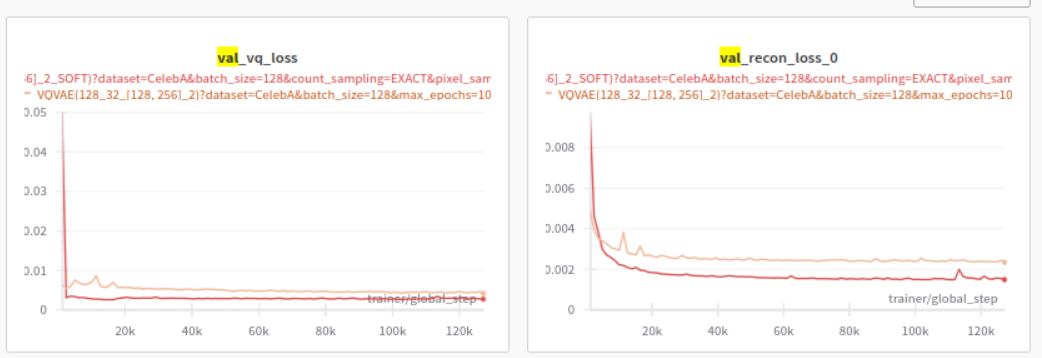
\includegraphics[width=0.8\textwidth]{figures/results/VQ+RECON.png}
    \caption[Validation loss comparison during training of a Gaussian VAE.]
    {
        Validation losses during training with and without \methodOne{1} applied on VQ-VAE.
        Left: VQ objective loss comparison. Right: Reconstruction loss comparison of the $Decoder_1$ - non-conditioned decoder.
    }
    \label{fig:results_method1_vq_vae}
\end{figure}

\section{Results of \methodTwo{2}}

In this section, I will present the results of \methodTwo{2} on both Gaussian VAEs and VQ-VAEs. The method was applied to the same datasets as the previous method. For this method, I ran the experiments with both Uniform and Gaussian sampling. The count sampling was done with Power law distribution with different exponent values.

\subsection{Results on Gaussian VAEs}

The results showed that \methodTwo{2} can be used for unifying two decoders into one. The experiments were conducted with both Uniform and Gaussian sampling. The results showed that for both methods this comes at a cost of slightly lower quality of the reconstruction when no conditioning information is given compared to a standard Gaussian VAE. However, the findings showed that this approach can substantially reduce the KL divergence loss of the latent space, which can be seen in figure \ref{fig:results_method2_gaussian_vae}.

Although, for both Uniform and Gaussian sampling findings showed that this method results in a slightly lower quality of the reconstruction compared to a standard Gaussian VAE. This approach reduced the KL divergence loss of the latent space for both of the sampling methods. For Uniform sampling, the results showed that the KL divergence loss of the latent space was reduced more compared to Gaussian sampling. One possible explanation for this could be that with Gaussian sampling, there is a higher probability of sampling the same pixel multiple times, which can be less informative for the decoder.

Experiments were also conducted with a range of different exponent values for the power-law distribution. The findings showed that the higher the exponent value the more the model was able to reduce the reconstruction loss of the scenario, where no conditioning information is given. However, the KL divergence loss of the latent space increased with higher exponent values.

\begin{figure}[H]
    \centering
    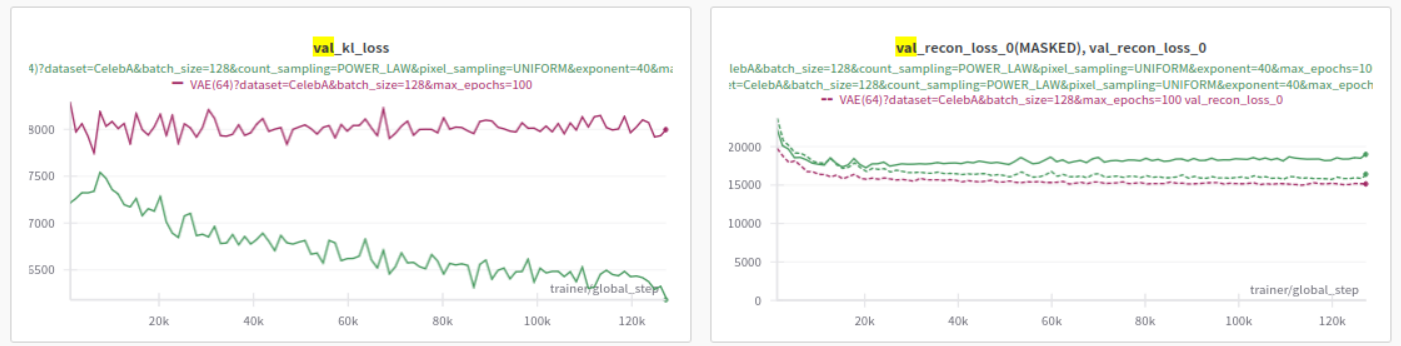
\includegraphics[width=0.8\textwidth]{figures/results/scvae1d/KL_and_recon.png}
    \caption[Validation loss during training with \methodTwo{2} applied on Gaussian VAE.]
    {
        Validation losses during training with and without \methodTwo{2} applied on Gaussian VAE.
        Left: KL loss comparison. Right: Reconstruction loss comparison of the $Decoder_1$ - non-conditioned decoder with a standard Gaussian VAE.
    }
    \label{fig:results_method2_gaussian_vae}
\end{figure}

\subsection{Results on VQ-VAEs}

The results showed that \methodTwo{2} worked very well with VQ-VAEs. The results showed it can be used to substantially reduce the VQ objective loss and at the same time to improve the quality of the reconstruction when no conditioning information is given. This showed to be the case for both Uniform and Gaussian sampling with a high enough exponent value for the power-law distribution.

The experiments were run with a range of different exponent values: 20, 30, 40, 50, 60. The results showed that the higher the exponent value the better the reconstruction in the scenario where no conditioning information is given, which is expected since the higher the exponent value the less number of pixels are given to the decoder as conditioning information on average.

When comparing Uniform and Gaussian sampling, the results showed that Gaussian sampling performed slightly better than Uniform sampling. This can be explained by the fact that the information around the center of the image is more important for the reconstruction, which is more likely to be sampled with Gaussian sampling.

\begin{figure}[H]
    \centering
    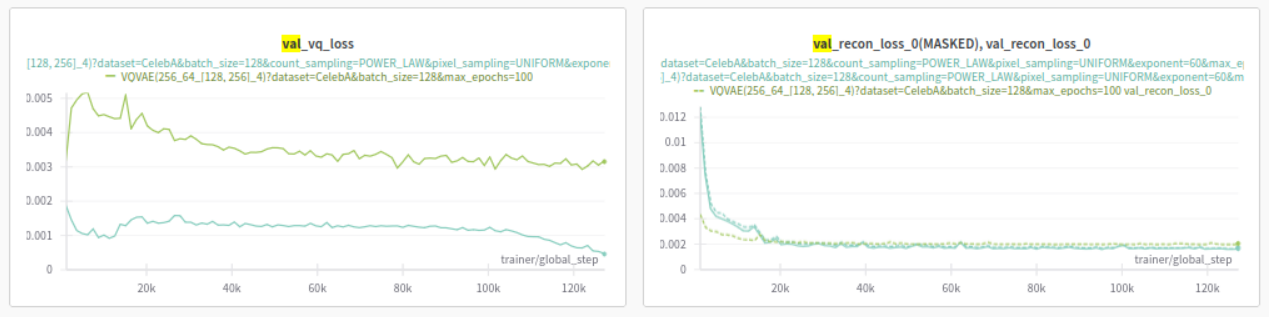
\includegraphics[width=0.8\textwidth]{figures/results/scvqvae1d/VQ_and_recon.png}
    \caption[Validation loss comparison during training of a VQ-VAE.]
    {
        Validation losses during training with and without \methodTwo{2} applied on VQ-VAE.
        Left: VQ objective loss comparison. Right: Reconstruction loss comparison of the $Decoder_1$ - non-conditioned decoder with a standard VQ-VAE.
    }
    \label{fig:results_method2_vq_vae}
\end{figure}

\section{Cross-validation results}

In this section, I will present the cross-validation results of both methods. The cross-validation was conducted on both Gaussian VAEs and VQ-VAEs. The cross-validation was conducted with 5 folds, where the data was split into 80\% training and 20\% validation.
The final cross-validation results are presented in table \ref{tab:cross_val_results}.

% Create a table with description
\begin{table}
    \centering
\scriptsize
\begin{tabular}{||c|c|c|c|c|c||}
\hline
 & Config. & Method & Parameters & Reconstruction loss & VQ/KL loss \\
\hline
\multirow{27}{*}{\rotatebox[origin=c]{90}{VQ-VAE}} & \multirow{9}{*}{1} & \multirow{1}{*}{-} & - & 0.0028 +- 8.8e-09 & 0.0101 +- 4.7e-07 \\
\cline{4-6}
\cline{3-6}
 &  & \multirow{4}{*}{Multi Decoder} & Exact sampling & 0.0025 +- 6.5e-09 & 0.0082 +- 1.9e-07 \\
\cline{4-6}
 &  &  & Exact sampling, SoftAdapt & 0.0123 +- 3.9e-04 & 0.0035 +- 2.3e-06 \\
\cline{4-6}
 &  &  & Uniform sampling & \textbf{0.0023 +- 2.4e-09} & 0.0076 +- 2.8e-07 \\
\cline{4-6}
 &  &  & Uniform sampling, SoftAdapt & 0.0024 +- 3.6e-08 & 0.0042 +- 2.4e-07 \\
\cline{4-6}
\cline{3-6}
 &  & \multirow{4}{*}{Single Decoder} & Gaussian sampling, Exponent=40 & 0.0028 +- 7.4e-08 & 0.0028 +- 2.0e-07 \\
\cline{4-6}
 &  &  & Gaussian sampling, Exponent=60 & 0.0029 +- 7.2e-08 & 0.0029 +- 1.3e-07 \\
\cline{4-6}
 &  &  & Uniform sampling, Exponent=40 & 0.0029 +- 6.4e-08 & 0.0030 +- 4.2e-07 \\
\cline{4-6}
 &  &  & Uniform sampling, Exponent=60 & 0.0030 +- 7.2e-08 & \textbf{0.0024 +- 2.4e-08} \\
\cline{4-6}
\cline{3-6}
\cline{2-6}
 & \multirow{9}{*}{3} & \multirow{1}{*}{-} & - & 0.0019 +- 1.3e-08 & 0.0024 +- 4.3e-08 \\
\cline{4-6}
\cline{3-6}
 &  & \multirow{4}{*}{Multi Decoder} & Exact sampling & 0.0017 +- 8.4e-09 & 0.0028 +- 1.2e-07 \\
\cline{4-6}
 &  &  & Exact sampling, SoftAdapt & 0.0173 +- 6.9e-04 & 0.0011 +- 2.2e-07 \\
\cline{4-6}
 &  &  & Uniform sampling & \textbf{0.0017 +- 2.4e-08} & 0.0024 +- 1.2e-07 \\
\cline{4-6}
 &  &  & Uniform sampling, SoftAdapt & 0.0178 +- 6.5e-04 & 0.0009 +- 2.8e-07 \\
\cline{4-6}
\cline{3-6}
 &  & \multirow{4}{*}{Single Decoder} & Gaussian sampling, Exponent=40 & 0.0038 +- 8.7e-08 & 0.0008 +- 2.4e-07 \\
\cline{4-6}
 &  &  & Gaussian sampling, Exponent=60 & 0.0037 +- 5.7e-08 & \textbf{0.0005 +- 1.1e-07} \\
\cline{4-6}
 &  &  & Uniform sampling, Exponent=40 & 0.0039 +- 1.1e-07 & 0.0007 +- 1.8e-08 \\
\cline{4-6}
 &  &  & Uniform sampling, Exponent=60 & 0.0038 +- 2.4e-08 & 0.0007 +- 4.0e-08 \\
\cline{4-6}
\cline{3-6}
\cline{2-6}
 & \multirow{9}{*}{2} & \multirow{1}{*}{-} & - & 0.0017 +- 1.6e-09 & 0.0022 +- 2.0e-08 \\
\cline{4-6}
\cline{3-6}
 &  & \multirow{4}{*}{Multi Decoder} & Exact sampling & \textbf{0.0014 +- 2.8e-09} & 0.0028 +- 3.3e-08 \\
\cline{4-6}
 &  &  & Exact sampling, SoftAdapt & 0.0155 +- 7.9e-04 & 0.0013 +- 3.6e-07 \\
\cline{4-6}
 &  &  & Uniform sampling & 0.0015 +- 2.7e-09 & 0.0030 +- 2.5e-08 \\
\cline{4-6}
 &  &  & Uniform sampling, SoftAdapt & 0.0422 +- 1.1e-03 & \textbf{0.0009 +- 3.2e-07} \\
\cline{4-6}
\cline{3-6}
 &  & \multirow{4}{*}{Single Decoder} & Gaussian sampling, Exponent=40 & 0.0031 +- 1.6e-07 & 0.0014 +- 3.5e-07 \\
\cline{4-6}
 &  &  & Gaussian sampling, Exponent=60 & 0.0031 +- 2.1e-07 & 0.0013 +- 2.6e-07 \\
\cline{4-6}
 &  &  & Uniform sampling, Exponent=40 & 0.0029 +- 1.4e-07 & 0.0017 +- 5.6e-08 \\
\cline{4-6}
 &  &  & Uniform sampling, Exponent=60 & 0.0035 +- 3.3e-07 & 0.0012 +- 4.3e-07 \\
\cline{4-6}
\cline{3-6}
\cline{2-6}
\hline
\multirow{18}{*}{\rotatebox[origin=c]{90}{Gaussian VAE}} & \multirow{9}{*}{1} & \multirow{1}{*}{-} & - & 0.0178 +- 1.2e-03 & 0.0165 +- 4.5e-03 \\
\cline{4-6}
\cline{3-6}
 &  & \multirow{4}{*}{Multi Decoder} & Exact sampling & 0.0145 +- 2.3e-03 & 0.0222 +- 1.2e-02 \\
\cline{4-6}
 &  &  & Exact sampling, SoftAdapt & 0.0168 +- 1.3e-03 & 0.0186 +- 1.3e-02 \\
\cline{4-6}
 &  &  & Uniform sampling & \textbf{0.0134 +- 5.4e-03} & 0.0234 +- 2.6e-02 \\
\cline{4-6}
 &  &  & Uniform sampling, SoftAdapt & 0.0158 +- 3.3e-03 & 0.0195 +- 3.9e-03 \\
\cline{4-6}
\cline{3-6}
 &  & \multirow{4}{*}{Single Decoder} & Gaussian sampling, Exponent=40 & 0.0204 +- 2.7e-02 & 0.0126 +- 6.8e-03 \\
\cline{4-6}
 &  &  & Gaussian sampling, Exponent=60 & 0.0203 +- 1.7e-02 & \textbf{0.0124 +- 2.9e-03} \\
\cline{4-6}
 &  &  & Uniform sampling, Exponent=40 & 0.0201 +- 9.6e-03 & 0.0148 +- 2.4e-03 \\
\cline{4-6}
 &  &  & Uniform sampling, Exponent=60 & 0.0202 +- 2.7e-02 & 0.0147 +- 3.0e-03 \\
\cline{4-6}
\cline{3-6}
\cline{2-6}
 & \multirow{9}{*}{2} & \multirow{1}{*}{-} & - & 0.0181 +- 8.7e-03 & 0.0161 +- 9.4e-03 \\
\cline{4-6}
\cline{3-6}
 &  & \multirow{4}{*}{Multi Decoder} & Exact sampling & 0.0148 +- 8.5e-03 & 0.0219 +- 7.5e-03 \\
\cline{4-6}
 &  &  & Exact sampling, SoftAdapt & 0.0167 +- 1.1e-02 & 0.0188 +- 3.7e-03 \\
\cline{4-6}
 &  &  & Uniform sampling & \textbf{0.0136 +- 8.8e-03} & 0.0235 +- 2.3e-02 \\
\cline{4-6}
 &  &  & Uniform sampling, SoftAdapt & 0.0158 +- 2.3e-03 & 0.0195 +- 4.8e-03 \\
\cline{4-6}
\cline{3-6}
 &  & \multirow{4}{*}{Single Decoder} & Gaussian sampling, Exponent=40 & 0.0209 +- 5.4e-02 & 0.0125 +- 1.0e-03 \\
\cline{4-6}
 &  &  & Gaussian sampling, Exponent=60 & 0.0207 +- 2.7e-02 & \textbf{0.0125 +- 4.0e-03} \\
\cline{4-6}
 &  &  & Uniform sampling, Exponent=40 & 0.0204 +- 3.4e-02 & 0.0147 +- 4.4e-03 \\
\cline{4-6}
 &  &  & Uniform sampling, Exponent=60 & 0.0204 +- 2.8e-02 & 0.0149 +- 5.3e-03 \\
\cline{4-6}
\cline{3-6}
\cline{2-6}
\hline
\hline
\end{tabular}

    \caption{Cross-validation results of \methodOne{1} and \methodTwo{2} on the MNIST dataset.}
    \label{tab:cross_val_results}
\end{table}